% lecture4_ro.tex -- GENERATED by build_L4.py from L4_numbers.json; do not edit by hand.
\documentclass[10pt,aspectratio=169,t]{beamer}
% =============================================================================
% nn_preamble.tex -- shared Beamer preamble of Neural Networks and Deep Learning (NN)
% Used by every lecture: lectures/Lk/lecturek.tex does
%   \documentclass[10pt,aspectratio=169,t]{beamer}
%   % =============================================================================
% nn_preamble.tex -- shared Beamer preamble of Neural Networks and Deep Learning (NN)
% Used by every lecture: lectures/Lk/lecturek.tex does
%   \documentclass[10pt,aspectratio=169,t]{beamer}
%   % =============================================================================
% nn_preamble.tex -- shared Beamer preamble of Neural Networks and Deep Learning (NN)
% Used by every lecture: lectures/Lk/lecturek.tex does
%   \documentclass[10pt,aspectratio=169,t]{beamer}
%   \input{../common/nn_preamble}
%   \nnlecture{k}{Lecture title}
% Logos live in lectures/common/logos/, charts in lectures/Lk/charts/.
% Do NOT add \hfuzz / \vfuzz / \hbadness here: overfull boxes must be fixed, not hidden.
% =============================================================================

\usetheme{default}
\setbeamersize{text margin left=7mm, text margin right=7mm}

% ---------------------------------------------------------------- packages
\usepackage[utf8]{inputenc}
\usepackage[T1]{fontenc}
\usepackage{lmodern}
\usepackage{amsmath, amssymb}
\usepackage{mathtools}
\usepackage{bm}
\usepackage{tikz}
\usetikzlibrary{arrows.meta, positioning, calc, shapes.misc}
\usepackage{booktabs}
\usepackage{array}
\usepackage{graphicx}
\usepackage{colortbl}
\usepackage{xcolor}
\usepackage{multicol}
\hypersetup{colorlinks=true, linkcolor=MainBlue, urlcolor=MainBlue, citecolor=MainBlue}
\graphicspath{{../common/logos/}}   % charts are included with their language folder: charts/en/, charts/ro/

% ---------------------------------------------------------------- colours
\definecolor{MainBlue}{RGB}{26, 58, 110}
\definecolor{IDAred}{RGB}{205, 0, 0}
\definecolor{DarkGray}{RGB}{51, 51, 51}
\definecolor{FooterGray}{RGB}{100, 100, 100}
\definecolor{BlockGray}{RGB}{236, 238, 242}
\definecolor{KeynoteGray}{RGB}{218, 218, 218}
\definecolor{Crimson}{RGB}{190, 40, 50}
\definecolor{Forest}{RGB}{30, 110, 50}
\definecolor{Bitter}{RGB}{214, 150, 20}
% chart palette (same hex values and order as lectures/common/nn_plot.py SERIES)
\definecolor{Ser1}{HTML}{2A78D6}
\definecolor{Ser2}{HTML}{EB6834}
\definecolor{Ser3}{HTML}{1BAF7A}
\definecolor{Ser4}{HTML}{EDA100}
\definecolor{Ser5}{HTML}{E87BA4}
\definecolor{Ser6}{HTML}{008300}
\definecolor{Ser7}{HTML}{6250D6}
\definecolor{Ser8}{HTML}{E34948}

\setbeamertemplate{background}{%
  \begin{tikzpicture}[remember picture, overlay]
    \shade[shading=axis, shading angle=315, top color=white, bottom color=KeynoteGray]
      (current page.south west) rectangle (current page.north east);
  \end{tikzpicture}}
\setbeamercolor{background canvas}{bg=}
\setbeamercolor{structure}{fg=MainBlue}
\setbeamercolor{normal text}{fg=DarkGray}
\setbeamercolor{title}{fg=IDAred}
\setbeamercolor{frametitle}{fg=IDAred, bg=}
\setbeamercolor{block title}{bg=MainBlue, fg=white}
\setbeamercolor{block body}{bg=BlockGray, fg=DarkGray}
\setbeamercolor{block title alerted}{bg=Crimson, fg=white}
\setbeamercolor{block body alerted}{bg=Crimson!7, fg=DarkGray}
\setbeamercolor{block title example}{bg=Forest, fg=white}
\setbeamercolor{block body example}{bg=Forest!7, fg=DarkGray}
\setbeamercolor{item}{fg=MainBlue}
\setbeamerfont{frametitle}{size=\large, series=\bfseries}
\setbeamerfont{block title}{size=\small, series=\bfseries}
\setbeamertemplate{blocks}[rounded][shadow=false]
\setbeamertemplate{itemize item}{\color{MainBlue}$\boxdot$}
\setbeamertemplate{itemize subitem}{\color{MainBlue}\scriptsize$\blacktriangleright$}
% compact two-level lists: level 1 = main point, level 2 = details (no text outside bullets)
\setbeamerfont{itemize/enumerate subbody}{size=\footnotesize}
\setlength{\leftmargini}{1.1em}
\setlength{\leftmarginii}{1.1em}
\setbeamertemplate{itemize/enumerate body begin}{\setlength{\topsep}{0pt}\setlength{\partopsep}{0pt}\setlength{\parskip}{0pt}}
\setbeamertemplate{itemize/enumerate subbody begin}{\setlength{\topsep}{0pt}\setlength{\partopsep}{0pt}\setlength{\itemsep}{0pt}\vspace{-0.4ex}}

\setbeamertemplate{enumerate item}{\color{MainBlue}\insertenumlabel.}
\setlength{\leftmargini}{1.3em}
\setlength{\leftmarginii}{1.2em}
\setbeamertemplate{navigation symbols}{}
\setbeamertemplate{section in toc}{\color{MainBlue}$\blacktriangleright$~\inserttocsection}
\setbeamertemplate{caption}{\raggedright\insertcaption\par}
% frame subtitle = precise citation line under the claim title (Weron style)
\setbeamerfont{framesubtitle}{size=\footnotesize}
\setbeamercolor{framesubtitle}{fg=FooterGray}
% outline that reappears at every section with the current section highlighted
\setbeamertemplate{section in toc shaded}[default][35]
\setbeamertemplate{subsection in toc shaded}[default][35]
\setbeamertemplate{subsection in toc}{\leavevmode\leftskip=2.2em\color{DarkGray}\small\inserttocsubsection\par}
\AtBeginSection[]{{\begin{frame}{\txtoutline}\vspace{2mm}\small
  \tableofcontents[currentsection,hideothersubsections]\end{frame}}}

% ---------------------------------------------------------------- head and foot
\setbeamertemplate{headline}{%
  \vskip10pt%
  \hbox to \paperwidth{\hskip0.5cm%
    {\small\color{FooterGray}\renewcommand{\hyperlink}[2]{##2}\insertsectionhead}%
    \hfill\textcolor{FooterGray}{\small\insertframenumber}\hskip0.5cm}%
  \vskip4pt{\color{FooterGray}\hrule height 0.4pt}}
% footer as in the other courses (MFM, SFM): course name on the left, small sparkline on the right
\setbeamertemplate{footline}{%
  {\color{FooterGray}\hrule height 0.4pt}\vskip4pt%
  \hbox to \paperwidth{\hskip0.5cm%
    \textcolor{FooterGray}{\small\txtcourse}%
    \hfill\raisebox{-0.1em}{\begin{tikzpicture}[x=0.08em, y=0.08em, line width=0.4pt]
      \draw[FooterGray] (0,3) -- (1,4) -- (2,3.5) -- (3,5) -- (4,4) -- (5,6) -- (6,5.5) -- (7,4) -- (8,5) -- (9,7) -- (10,6) -- (11,5) -- (12,6.5) -- (13,8) -- (14,7) -- (15,6) -- (16,7.5) -- (17,9) -- (18,8) -- (19,7) -- (20,8.5) -- (21,10) -- (22,9) -- (23,8) -- (24,9.5);
    \end{tikzpicture}}\hskip0.5cm}%
  \vskip6pt}

% ---------------------------------------------------------------- title page
\defbeamertemplate*{title page}{nn}[1][]{%
  \vspace{0.15cm}
  \begin{center}
    \href{https://www.ase.ro}{
\includegraphics[height=0.9cm]{ase_logo.png}}\hspace{0.3cm}%
    \href{https://ipe.ro/new}{
\includegraphics[height=0.9cm]{acad_logo.png}}\hspace{0.3cm}%
    \href{https://theida.net}{
\includegraphics[height=0.9cm]{ida_logo.png}}\hspace{0.3cm}%
    \href{https://blockchain-research-center.com}{
\includegraphics[height=0.9cm]{brc_logo.png}}\hspace{0.3cm}%
    \href{https://www.ai4efin.ase.ro}{
\includegraphics[height=0.9cm]{ai4efin_logo.png}}\hspace{0.3cm}%
    \href{https://www.digital-finance-msca.com}{
\includegraphics[height=0.9cm]{msca_logo.png}}%
  \end{center}
  \vspace{0.45cm}
  \begin{center}
    \begin{minipage}{0.1\textwidth}\centering
      \href{https://quantlet.com}{
\includegraphics[height=0.9cm]{ql_logo.png}}\end{minipage}%
    \begin{minipage}{0.78\textwidth}\centering
      {\Large\bfseries\usebeamercolor[fg]{title}\inserttitle}\par\vspace{0.25cm}
      {\large\usebeamercolor[fg]{title}\insertsubtitle}\end{minipage}%
    \begin{minipage}{0.1\textwidth}\centering
      \href{https://quantinar.com}{
\includegraphics[height=0.9cm]{qr_logo.png}}\end{minipage}
  \end{center}
  \vfill
  \hspace{0.4cm}{\bfseries\insertauthor}\par\vspace{0.12cm}
  \hspace{0.4cm}\begin{minipage}[t]{0.92\textwidth}\raggedright\footnotesize\insertinstitute\end{minipage}
  \par\vspace{0.4cm}}

% ---------------------------------------------------------------- lecture metadata
\newcommand{\nnshort}{}
\newcommand{\nnnb}{notebooks}
\newcommand{\nnrepo}{https://github.com/danpele/NEURAL_BIZ/tree/main}
% language-dependent labels (English default; \nnromanian switches to Romanian, call it before \nnlecture)
\newcommand{\txtcourse}{Neural Networks and Deep Learning}
\newcommand{\txtlecture}{Lecture}
\newcommand{\txtoutline}{Outline}
\newcommand{\txtintuition}{In one sentence:}
\newcommand{\txtjob}{In practice:}
\newcommand{\txttry}{Experiment yourself:}
\newcommand{\txtwhere}{where}
\newcommand{\txtsim}{SIMULATED DATA (teaching illustration)}
\newcommand{\txtnbsuffix}{}
\newcommand{\txtinstitute}{Bucharest University of Economic Studies (ASE), Department of Statistics and Econometrics\\
    Romanian Academy, Institute for Economic Forecasting (IPE)\\
    IDA Institute Digital Assets \textbullet\ AI4EFin \textbullet\ MSCA Digital Finance}
\newcommand{\nnromanian}{%
  \renewcommand{\txtcourse}{Rețele neuronale și deep learning}%
  \renewcommand{\txtlecture}{Cursul}%
  \renewcommand{\txtoutline}{Cuprins}%
  \renewcommand{\txtintuition}{Pe scurt:}%
  \renewcommand{\txtjob}{În practică:}%
  \renewcommand{\txttry}{Exercițiu practic:}%
  \renewcommand{\txtwhere}{unde}%
  \renewcommand{\txtsim}{DATE SIMULATE (doar pentru ilustrare)}%
  \renewcommand{\txtnbsuffix}{\string_ro}%
  \renewcommand{\txtinstitute}{Academia de Studii Economice din București (ASE), Departamentul de Statistică și Econometrie\\
    Academia Română, Institutul de Prognoză Economică (IPE)\\
    IDA Institute Digital Assets \textbullet\ AI4EFin \textbullet\ MSCA Digital Finance}}
\newcommand{\nnlecture}[2]{%
  \renewcommand{\nnshort}{\txtlecture\ #1}%
  \renewcommand{\nnnb}{notebooks/L#1\string_notebook\txtnbsuffix.ipynb}%
  \title[NN]{\txtcourse}%
  \subtitle{\txtlecture\ #1: #2}%
  \author{Prof.\ dr.\ Daniel Traian PELE}%
  \institute{\txtinstitute}%
  \date{}}

% ---------------------------------------------------------------- teaching blocks (one message per frame)
% \intuition{one plain sentence}  ->  formula with every symbol defined  ->  real-data example  ->  \manager{one line}
\newcommand{\intuition}[1]{\begin{itemize}\item {\color{MainBlue}\textbf{\txtintuition}}~#1\end{itemize}\vspace{0.6mm}}
\newcommand{\manager}[1]{\colorbox{Forest!10}{\parbox{\dimexpr\linewidth-2\fboxsep\relax}{\footnotesize
  \begin{itemize}\setlength{\itemsep}{0pt}\item \textbf{\color{Forest}\txtjob}~#1\end{itemize}}}}
% Experiment yourself: pointer to the matching notebook section
\newcommand{\tryit}[1]{{\scriptsize\href{\nnrepo/\nnnb}{%
  \raisebox{-0.15em}{
\includegraphics[height=0.85em]{ql_logo.png}}\,\textbf{\txttry}~\color{MainBlue}#1}}}
% bottom row: manager line (left) + experiment pointer (right), pinned to the bottom of the frame
\newcommand{\bottomrow}[2]{\par\vfill\noindent\begin{minipage}[b]{0.72\linewidth}#1\end{minipage}\hfill
  \begin{minipage}[b]{0.26\linewidth}\raggedleft #2\end{minipage}\par\vspace{0.5mm}}
\newcommand{\where}[1]{{\footnotesize\textbf{\txtwhere}~#1\par}}

% ---------------------------------------------------------------- helpers
% chart source line under a figure: \chartsource{Source ...; period ...}
\newcommand{\chartsource}[1]{\par\vspace{1pt}{\scriptsize\color{FooterGray}#1\par}}
% link to code: \quantlet{label}{path inside the repo}
\newcommand{\quantlet}[2]{\par\vspace{1pt}\hfill\href{\nnrepo/#2}{%
  \raisebox{-0.15em}{
\includegraphics[height=0.75em]{ql_logo.png}}\textcolor{MainBlue}{\scriptsize\ #1}}}
% inline Quantlet link for the bottom-right corner of a frame: \qlink{label}{path inside the repo}
\newcommand{\qlink}[2]{{\scriptsize\href{\nnrepo/#2}{\raisebox{-0.15em}{
\includegraphics[height=0.85em]{ql_logo.png}}\,\textcolor{MainBlue}{#1}}}}
\newcommand{\simlabel}{\colorbox{Crimson!12}{\scriptsize\bfseries\color{Crimson}\txtsim}}
\newcommand{\E}{\mathbb{E}}
\newcommand{\Var}{\operatorname{Var}}
\newcommand{\Cov}{\operatorname{Cov}}
\newcommand{\Corr}{\operatorname{Corr}}
\newcommand{\asinh}{\operatorname{asinh}}
\newcommand{\iid}{\overset{\text{i.i.d.}}{\sim}}
\newcommand{\EUR}{EUR}
% deep-learning notation (Bishop & Bishop, 2024): vectors bold lower case, matrices bold upper case
\newcommand{\R}{\mathbb{R}}
\newcommand{\vx}{\mathbf{x}}
\newcommand{\vy}{\mathbf{y}}
\newcommand{\vz}{\mathbf{z}}
\newcommand{\vh}{\mathbf{h}}
\newcommand{\vw}{\mathbf{w}}
\newcommand{\vb}{\mathbf{b}}
\newcommand{\mW}{\mathbf{W}}
\newcommand{\mX}{\mathbf{X}}
\newcommand{\btheta}{\boldsymbol{\theta}}
\newcommand{\loss}{\mathcal{L}}
\newcommand{\dataset}{\mathcal{D}}
\DeclareMathOperator*{\argmin}{arg\,min}
\DeclareMathOperator*{\argmax}{arg\,max}
\DeclareMathOperator{\softmax}{softmax}
\DeclareMathOperator{\ReLU}{ReLU}
\DeclareMathOperator{\sigm}{\sigma}

%   \nnlecture{k}{Lecture title}
% Logos live in lectures/common/logos/, charts in lectures/Lk/charts/.
% Do NOT add \hfuzz / \vfuzz / \hbadness here: overfull boxes must be fixed, not hidden.
% =============================================================================

\usetheme{default}
\setbeamersize{text margin left=7mm, text margin right=7mm}

% ---------------------------------------------------------------- packages
\usepackage[utf8]{inputenc}
\usepackage[T1]{fontenc}
\usepackage{lmodern}
\usepackage{amsmath, amssymb}
\usepackage{mathtools}
\usepackage{bm}
\usepackage{tikz}
\usetikzlibrary{arrows.meta, positioning, calc, shapes.misc}
\usepackage{booktabs}
\usepackage{array}
\usepackage{graphicx}
\usepackage{colortbl}
\usepackage{xcolor}
\usepackage{multicol}
\hypersetup{colorlinks=true, linkcolor=MainBlue, urlcolor=MainBlue, citecolor=MainBlue}
\graphicspath{{../common/logos/}}   % charts are included with their language folder: charts/en/, charts/ro/

% ---------------------------------------------------------------- colours
\definecolor{MainBlue}{RGB}{26, 58, 110}
\definecolor{IDAred}{RGB}{205, 0, 0}
\definecolor{DarkGray}{RGB}{51, 51, 51}
\definecolor{FooterGray}{RGB}{100, 100, 100}
\definecolor{BlockGray}{RGB}{236, 238, 242}
\definecolor{KeynoteGray}{RGB}{218, 218, 218}
\definecolor{Crimson}{RGB}{190, 40, 50}
\definecolor{Forest}{RGB}{30, 110, 50}
\definecolor{Bitter}{RGB}{214, 150, 20}
% chart palette (same hex values and order as lectures/common/nn_plot.py SERIES)
\definecolor{Ser1}{HTML}{2A78D6}
\definecolor{Ser2}{HTML}{EB6834}
\definecolor{Ser3}{HTML}{1BAF7A}
\definecolor{Ser4}{HTML}{EDA100}
\definecolor{Ser5}{HTML}{E87BA4}
\definecolor{Ser6}{HTML}{008300}
\definecolor{Ser7}{HTML}{6250D6}
\definecolor{Ser8}{HTML}{E34948}

\setbeamertemplate{background}{%
  \begin{tikzpicture}[remember picture, overlay]
    \shade[shading=axis, shading angle=315, top color=white, bottom color=KeynoteGray]
      (current page.south west) rectangle (current page.north east);
  \end{tikzpicture}}
\setbeamercolor{background canvas}{bg=}
\setbeamercolor{structure}{fg=MainBlue}
\setbeamercolor{normal text}{fg=DarkGray}
\setbeamercolor{title}{fg=IDAred}
\setbeamercolor{frametitle}{fg=IDAred, bg=}
\setbeamercolor{block title}{bg=MainBlue, fg=white}
\setbeamercolor{block body}{bg=BlockGray, fg=DarkGray}
\setbeamercolor{block title alerted}{bg=Crimson, fg=white}
\setbeamercolor{block body alerted}{bg=Crimson!7, fg=DarkGray}
\setbeamercolor{block title example}{bg=Forest, fg=white}
\setbeamercolor{block body example}{bg=Forest!7, fg=DarkGray}
\setbeamercolor{item}{fg=MainBlue}
\setbeamerfont{frametitle}{size=\large, series=\bfseries}
\setbeamerfont{block title}{size=\small, series=\bfseries}
\setbeamertemplate{blocks}[rounded][shadow=false]
\setbeamertemplate{itemize item}{\color{MainBlue}$\boxdot$}
\setbeamertemplate{itemize subitem}{\color{MainBlue}\scriptsize$\blacktriangleright$}
% compact two-level lists: level 1 = main point, level 2 = details (no text outside bullets)
\setbeamerfont{itemize/enumerate subbody}{size=\footnotesize}
\setlength{\leftmargini}{1.1em}
\setlength{\leftmarginii}{1.1em}
\setbeamertemplate{itemize/enumerate body begin}{\setlength{\topsep}{0pt}\setlength{\partopsep}{0pt}\setlength{\parskip}{0pt}}
\setbeamertemplate{itemize/enumerate subbody begin}{\setlength{\topsep}{0pt}\setlength{\partopsep}{0pt}\setlength{\itemsep}{0pt}\vspace{-0.4ex}}

\setbeamertemplate{enumerate item}{\color{MainBlue}\insertenumlabel.}
\setlength{\leftmargini}{1.3em}
\setlength{\leftmarginii}{1.2em}
\setbeamertemplate{navigation symbols}{}
\setbeamertemplate{section in toc}{\color{MainBlue}$\blacktriangleright$~\inserttocsection}
\setbeamertemplate{caption}{\raggedright\insertcaption\par}
% frame subtitle = precise citation line under the claim title (Weron style)
\setbeamerfont{framesubtitle}{size=\footnotesize}
\setbeamercolor{framesubtitle}{fg=FooterGray}
% outline that reappears at every section with the current section highlighted
\setbeamertemplate{section in toc shaded}[default][35]
\setbeamertemplate{subsection in toc shaded}[default][35]
\setbeamertemplate{subsection in toc}{\leavevmode\leftskip=2.2em\color{DarkGray}\small\inserttocsubsection\par}
\AtBeginSection[]{{\begin{frame}{\txtoutline}\vspace{2mm}\small
  \tableofcontents[currentsection,hideothersubsections]\end{frame}}}

% ---------------------------------------------------------------- head and foot
\setbeamertemplate{headline}{%
  \vskip10pt%
  \hbox to \paperwidth{\hskip0.5cm%
    {\small\color{FooterGray}\renewcommand{\hyperlink}[2]{##2}\insertsectionhead}%
    \hfill\textcolor{FooterGray}{\small\insertframenumber}\hskip0.5cm}%
  \vskip4pt{\color{FooterGray}\hrule height 0.4pt}}
% footer as in the other courses (MFM, SFM): course name on the left, small sparkline on the right
\setbeamertemplate{footline}{%
  {\color{FooterGray}\hrule height 0.4pt}\vskip4pt%
  \hbox to \paperwidth{\hskip0.5cm%
    \textcolor{FooterGray}{\small\txtcourse}%
    \hfill\raisebox{-0.1em}{\begin{tikzpicture}[x=0.08em, y=0.08em, line width=0.4pt]
      \draw[FooterGray] (0,3) -- (1,4) -- (2,3.5) -- (3,5) -- (4,4) -- (5,6) -- (6,5.5) -- (7,4) -- (8,5) -- (9,7) -- (10,6) -- (11,5) -- (12,6.5) -- (13,8) -- (14,7) -- (15,6) -- (16,7.5) -- (17,9) -- (18,8) -- (19,7) -- (20,8.5) -- (21,10) -- (22,9) -- (23,8) -- (24,9.5);
    \end{tikzpicture}}\hskip0.5cm}%
  \vskip6pt}

% ---------------------------------------------------------------- title page
\defbeamertemplate*{title page}{nn}[1][]{%
  \vspace{0.15cm}
  \begin{center}
    \href{https://www.ase.ro}{
\includegraphics[height=0.9cm]{ase_logo.png}}\hspace{0.3cm}%
    \href{https://ipe.ro/new}{
\includegraphics[height=0.9cm]{acad_logo.png}}\hspace{0.3cm}%
    \href{https://theida.net}{
\includegraphics[height=0.9cm]{ida_logo.png}}\hspace{0.3cm}%
    \href{https://blockchain-research-center.com}{
\includegraphics[height=0.9cm]{brc_logo.png}}\hspace{0.3cm}%
    \href{https://www.ai4efin.ase.ro}{
\includegraphics[height=0.9cm]{ai4efin_logo.png}}\hspace{0.3cm}%
    \href{https://www.digital-finance-msca.com}{
\includegraphics[height=0.9cm]{msca_logo.png}}%
  \end{center}
  \vspace{0.45cm}
  \begin{center}
    \begin{minipage}{0.1\textwidth}\centering
      \href{https://quantlet.com}{
\includegraphics[height=0.9cm]{ql_logo.png}}\end{minipage}%
    \begin{minipage}{0.78\textwidth}\centering
      {\Large\bfseries\usebeamercolor[fg]{title}\inserttitle}\par\vspace{0.25cm}
      {\large\usebeamercolor[fg]{title}\insertsubtitle}\end{minipage}%
    \begin{minipage}{0.1\textwidth}\centering
      \href{https://quantinar.com}{
\includegraphics[height=0.9cm]{qr_logo.png}}\end{minipage}
  \end{center}
  \vfill
  \hspace{0.4cm}{\bfseries\insertauthor}\par\vspace{0.12cm}
  \hspace{0.4cm}\begin{minipage}[t]{0.92\textwidth}\raggedright\footnotesize\insertinstitute\end{minipage}
  \par\vspace{0.4cm}}

% ---------------------------------------------------------------- lecture metadata
\newcommand{\nnshort}{}
\newcommand{\nnnb}{notebooks}
\newcommand{\nnrepo}{https://github.com/danpele/NEURAL_BIZ/tree/main}
% language-dependent labels (English default; \nnromanian switches to Romanian, call it before \nnlecture)
\newcommand{\txtcourse}{Neural Networks and Deep Learning}
\newcommand{\txtlecture}{Lecture}
\newcommand{\txtoutline}{Outline}
\newcommand{\txtintuition}{In one sentence:}
\newcommand{\txtjob}{In practice:}
\newcommand{\txttry}{Experiment yourself:}
\newcommand{\txtwhere}{where}
\newcommand{\txtsim}{SIMULATED DATA (teaching illustration)}
\newcommand{\txtnbsuffix}{}
\newcommand{\txtinstitute}{Bucharest University of Economic Studies (ASE), Department of Statistics and Econometrics\\
    Romanian Academy, Institute for Economic Forecasting (IPE)\\
    IDA Institute Digital Assets \textbullet\ AI4EFin \textbullet\ MSCA Digital Finance}
\newcommand{\nnromanian}{%
  \renewcommand{\txtcourse}{Rețele neuronale și deep learning}%
  \renewcommand{\txtlecture}{Cursul}%
  \renewcommand{\txtoutline}{Cuprins}%
  \renewcommand{\txtintuition}{Pe scurt:}%
  \renewcommand{\txtjob}{În practică:}%
  \renewcommand{\txttry}{Exercițiu practic:}%
  \renewcommand{\txtwhere}{unde}%
  \renewcommand{\txtsim}{DATE SIMULATE (doar pentru ilustrare)}%
  \renewcommand{\txtnbsuffix}{\string_ro}%
  \renewcommand{\txtinstitute}{Academia de Studii Economice din București (ASE), Departamentul de Statistică și Econometrie\\
    Academia Română, Institutul de Prognoză Economică (IPE)\\
    IDA Institute Digital Assets \textbullet\ AI4EFin \textbullet\ MSCA Digital Finance}}
\newcommand{\nnlecture}[2]{%
  \renewcommand{\nnshort}{\txtlecture\ #1}%
  \renewcommand{\nnnb}{notebooks/L#1\string_notebook\txtnbsuffix.ipynb}%
  \title[NN]{\txtcourse}%
  \subtitle{\txtlecture\ #1: #2}%
  \author{Prof.\ dr.\ Daniel Traian PELE}%
  \institute{\txtinstitute}%
  \date{}}

% ---------------------------------------------------------------- teaching blocks (one message per frame)
% \intuition{one plain sentence}  ->  formula with every symbol defined  ->  real-data example  ->  \manager{one line}
\newcommand{\intuition}[1]{\begin{itemize}\item {\color{MainBlue}\textbf{\txtintuition}}~#1\end{itemize}\vspace{0.6mm}}
\newcommand{\manager}[1]{\colorbox{Forest!10}{\parbox{\dimexpr\linewidth-2\fboxsep\relax}{\footnotesize
  \begin{itemize}\setlength{\itemsep}{0pt}\item \textbf{\color{Forest}\txtjob}~#1\end{itemize}}}}
% Experiment yourself: pointer to the matching notebook section
\newcommand{\tryit}[1]{{\scriptsize\href{\nnrepo/\nnnb}{%
  \raisebox{-0.15em}{
\includegraphics[height=0.85em]{ql_logo.png}}\,\textbf{\txttry}~\color{MainBlue}#1}}}
% bottom row: manager line (left) + experiment pointer (right), pinned to the bottom of the frame
\newcommand{\bottomrow}[2]{\par\vfill\noindent\begin{minipage}[b]{0.72\linewidth}#1\end{minipage}\hfill
  \begin{minipage}[b]{0.26\linewidth}\raggedleft #2\end{minipage}\par\vspace{0.5mm}}
\newcommand{\where}[1]{{\footnotesize\textbf{\txtwhere}~#1\par}}

% ---------------------------------------------------------------- helpers
% chart source line under a figure: \chartsource{Source ...; period ...}
\newcommand{\chartsource}[1]{\par\vspace{1pt}{\scriptsize\color{FooterGray}#1\par}}
% link to code: \quantlet{label}{path inside the repo}
\newcommand{\quantlet}[2]{\par\vspace{1pt}\hfill\href{\nnrepo/#2}{%
  \raisebox{-0.15em}{
\includegraphics[height=0.75em]{ql_logo.png}}\textcolor{MainBlue}{\scriptsize\ #1}}}
% inline Quantlet link for the bottom-right corner of a frame: \qlink{label}{path inside the repo}
\newcommand{\qlink}[2]{{\scriptsize\href{\nnrepo/#2}{\raisebox{-0.15em}{
\includegraphics[height=0.85em]{ql_logo.png}}\,\textcolor{MainBlue}{#1}}}}
\newcommand{\simlabel}{\colorbox{Crimson!12}{\scriptsize\bfseries\color{Crimson}\txtsim}}
\newcommand{\E}{\mathbb{E}}
\newcommand{\Var}{\operatorname{Var}}
\newcommand{\Cov}{\operatorname{Cov}}
\newcommand{\Corr}{\operatorname{Corr}}
\newcommand{\asinh}{\operatorname{asinh}}
\newcommand{\iid}{\overset{\text{i.i.d.}}{\sim}}
\newcommand{\EUR}{EUR}
% deep-learning notation (Bishop & Bishop, 2024): vectors bold lower case, matrices bold upper case
\newcommand{\R}{\mathbb{R}}
\newcommand{\vx}{\mathbf{x}}
\newcommand{\vy}{\mathbf{y}}
\newcommand{\vz}{\mathbf{z}}
\newcommand{\vh}{\mathbf{h}}
\newcommand{\vw}{\mathbf{w}}
\newcommand{\vb}{\mathbf{b}}
\newcommand{\mW}{\mathbf{W}}
\newcommand{\mX}{\mathbf{X}}
\newcommand{\btheta}{\boldsymbol{\theta}}
\newcommand{\loss}{\mathcal{L}}
\newcommand{\dataset}{\mathcal{D}}
\DeclareMathOperator*{\argmin}{arg\,min}
\DeclareMathOperator*{\argmax}{arg\,max}
\DeclareMathOperator{\softmax}{softmax}
\DeclareMathOperator{\ReLU}{ReLU}
\DeclareMathOperator{\sigm}{\sigma}

%   \nnlecture{k}{Lecture title}
% Logos live in lectures/common/logos/, charts in lectures/Lk/charts/.
% Do NOT add \hfuzz / \vfuzz / \hbadness here: overfull boxes must be fixed, not hidden.
% =============================================================================

\usetheme{default}
\setbeamersize{text margin left=7mm, text margin right=7mm}

% ---------------------------------------------------------------- packages
\usepackage[utf8]{inputenc}
\usepackage[T1]{fontenc}
\usepackage{lmodern}
\usepackage{amsmath, amssymb}
\usepackage{mathtools}
\usepackage{bm}
\usepackage{tikz}
\usetikzlibrary{arrows.meta, positioning, calc, shapes.misc}
\usepackage{booktabs}
\usepackage{array}
\usepackage{graphicx}
\usepackage{colortbl}
\usepackage{xcolor}
\usepackage{multicol}
\hypersetup{colorlinks=true, linkcolor=MainBlue, urlcolor=MainBlue, citecolor=MainBlue}
\graphicspath{{../common/logos/}}   % charts are included with their language folder: charts/en/, charts/ro/

% ---------------------------------------------------------------- colours
\definecolor{MainBlue}{RGB}{26, 58, 110}
\definecolor{IDAred}{RGB}{205, 0, 0}
\definecolor{DarkGray}{RGB}{51, 51, 51}
\definecolor{FooterGray}{RGB}{100, 100, 100}
\definecolor{BlockGray}{RGB}{236, 238, 242}
\definecolor{KeynoteGray}{RGB}{218, 218, 218}
\definecolor{Crimson}{RGB}{190, 40, 50}
\definecolor{Forest}{RGB}{30, 110, 50}
\definecolor{Bitter}{RGB}{214, 150, 20}
% chart palette (same hex values and order as lectures/common/nn_plot.py SERIES)
\definecolor{Ser1}{HTML}{2A78D6}
\definecolor{Ser2}{HTML}{EB6834}
\definecolor{Ser3}{HTML}{1BAF7A}
\definecolor{Ser4}{HTML}{EDA100}
\definecolor{Ser5}{HTML}{E87BA4}
\definecolor{Ser6}{HTML}{008300}
\definecolor{Ser7}{HTML}{6250D6}
\definecolor{Ser8}{HTML}{E34948}

\setbeamertemplate{background}{%
  \begin{tikzpicture}[remember picture, overlay]
    \shade[shading=axis, shading angle=315, top color=white, bottom color=KeynoteGray]
      (current page.south west) rectangle (current page.north east);
  \end{tikzpicture}}
\setbeamercolor{background canvas}{bg=}
\setbeamercolor{structure}{fg=MainBlue}
\setbeamercolor{normal text}{fg=DarkGray}
\setbeamercolor{title}{fg=IDAred}
\setbeamercolor{frametitle}{fg=IDAred, bg=}
\setbeamercolor{block title}{bg=MainBlue, fg=white}
\setbeamercolor{block body}{bg=BlockGray, fg=DarkGray}
\setbeamercolor{block title alerted}{bg=Crimson, fg=white}
\setbeamercolor{block body alerted}{bg=Crimson!7, fg=DarkGray}
\setbeamercolor{block title example}{bg=Forest, fg=white}
\setbeamercolor{block body example}{bg=Forest!7, fg=DarkGray}
\setbeamercolor{item}{fg=MainBlue}
\setbeamerfont{frametitle}{size=\large, series=\bfseries}
\setbeamerfont{block title}{size=\small, series=\bfseries}
\setbeamertemplate{blocks}[rounded][shadow=false]
\setbeamertemplate{itemize item}{\color{MainBlue}$\boxdot$}
\setbeamertemplate{itemize subitem}{\color{MainBlue}\scriptsize$\blacktriangleright$}
% compact two-level lists: level 1 = main point, level 2 = details (no text outside bullets)
\setbeamerfont{itemize/enumerate subbody}{size=\footnotesize}
\setlength{\leftmargini}{1.1em}
\setlength{\leftmarginii}{1.1em}
\setbeamertemplate{itemize/enumerate body begin}{\setlength{\topsep}{0pt}\setlength{\partopsep}{0pt}\setlength{\parskip}{0pt}}
\setbeamertemplate{itemize/enumerate subbody begin}{\setlength{\topsep}{0pt}\setlength{\partopsep}{0pt}\setlength{\itemsep}{0pt}\vspace{-0.4ex}}

\setbeamertemplate{enumerate item}{\color{MainBlue}\insertenumlabel.}
\setlength{\leftmargini}{1.3em}
\setlength{\leftmarginii}{1.2em}
\setbeamertemplate{navigation symbols}{}
\setbeamertemplate{section in toc}{\color{MainBlue}$\blacktriangleright$~\inserttocsection}
\setbeamertemplate{caption}{\raggedright\insertcaption\par}
% frame subtitle = precise citation line under the claim title (Weron style)
\setbeamerfont{framesubtitle}{size=\footnotesize}
\setbeamercolor{framesubtitle}{fg=FooterGray}
% outline that reappears at every section with the current section highlighted
\setbeamertemplate{section in toc shaded}[default][35]
\setbeamertemplate{subsection in toc shaded}[default][35]
\setbeamertemplate{subsection in toc}{\leavevmode\leftskip=2.2em\color{DarkGray}\small\inserttocsubsection\par}
\AtBeginSection[]{{\begin{frame}{\txtoutline}\vspace{2mm}\small
  \tableofcontents[currentsection,hideothersubsections]\end{frame}}}

% ---------------------------------------------------------------- head and foot
\setbeamertemplate{headline}{%
  \vskip10pt%
  \hbox to \paperwidth{\hskip0.5cm%
    {\small\color{FooterGray}\renewcommand{\hyperlink}[2]{##2}\insertsectionhead}%
    \hfill\textcolor{FooterGray}{\small\insertframenumber}\hskip0.5cm}%
  \vskip4pt{\color{FooterGray}\hrule height 0.4pt}}
% footer as in the other courses (MFM, SFM): course name on the left, small sparkline on the right
\setbeamertemplate{footline}{%
  {\color{FooterGray}\hrule height 0.4pt}\vskip4pt%
  \hbox to \paperwidth{\hskip0.5cm%
    \textcolor{FooterGray}{\small\txtcourse}%
    \hfill\raisebox{-0.1em}{\begin{tikzpicture}[x=0.08em, y=0.08em, line width=0.4pt]
      \draw[FooterGray] (0,3) -- (1,4) -- (2,3.5) -- (3,5) -- (4,4) -- (5,6) -- (6,5.5) -- (7,4) -- (8,5) -- (9,7) -- (10,6) -- (11,5) -- (12,6.5) -- (13,8) -- (14,7) -- (15,6) -- (16,7.5) -- (17,9) -- (18,8) -- (19,7) -- (20,8.5) -- (21,10) -- (22,9) -- (23,8) -- (24,9.5);
    \end{tikzpicture}}\hskip0.5cm}%
  \vskip6pt}

% ---------------------------------------------------------------- title page
\defbeamertemplate*{title page}{nn}[1][]{%
  \vspace{0.15cm}
  \begin{center}
    \href{https://www.ase.ro}{
\includegraphics[height=0.9cm]{ase_logo.png}}\hspace{0.3cm}%
    \href{https://ipe.ro/new}{
\includegraphics[height=0.9cm]{acad_logo.png}}\hspace{0.3cm}%
    \href{https://theida.net}{
\includegraphics[height=0.9cm]{ida_logo.png}}\hspace{0.3cm}%
    \href{https://blockchain-research-center.com}{
\includegraphics[height=0.9cm]{brc_logo.png}}\hspace{0.3cm}%
    \href{https://www.ai4efin.ase.ro}{
\includegraphics[height=0.9cm]{ai4efin_logo.png}}\hspace{0.3cm}%
    \href{https://www.digital-finance-msca.com}{
\includegraphics[height=0.9cm]{msca_logo.png}}%
  \end{center}
  \vspace{0.45cm}
  \begin{center}
    \begin{minipage}{0.1\textwidth}\centering
      \href{https://quantlet.com}{
\includegraphics[height=0.9cm]{ql_logo.png}}\end{minipage}%
    \begin{minipage}{0.78\textwidth}\centering
      {\Large\bfseries\usebeamercolor[fg]{title}\inserttitle}\par\vspace{0.25cm}
      {\large\usebeamercolor[fg]{title}\insertsubtitle}\end{minipage}%
    \begin{minipage}{0.1\textwidth}\centering
      \href{https://quantinar.com}{
\includegraphics[height=0.9cm]{qr_logo.png}}\end{minipage}
  \end{center}
  \vfill
  \hspace{0.4cm}{\bfseries\insertauthor}\par\vspace{0.12cm}
  \hspace{0.4cm}\begin{minipage}[t]{0.92\textwidth}\raggedright\footnotesize\insertinstitute\end{minipage}
  \par\vspace{0.4cm}}

% ---------------------------------------------------------------- lecture metadata
\newcommand{\nnshort}{}
\newcommand{\nnnb}{notebooks}
\newcommand{\nnrepo}{https://github.com/danpele/NEURAL_BIZ/tree/main}
% language-dependent labels (English default; \nnromanian switches to Romanian, call it before \nnlecture)
\newcommand{\txtcourse}{Neural Networks and Deep Learning}
\newcommand{\txtlecture}{Lecture}
\newcommand{\txtoutline}{Outline}
\newcommand{\txtintuition}{In one sentence:}
\newcommand{\txtjob}{In practice:}
\newcommand{\txttry}{Experiment yourself:}
\newcommand{\txtwhere}{where}
\newcommand{\txtsim}{SIMULATED DATA (teaching illustration)}
\newcommand{\txtnbsuffix}{}
\newcommand{\txtinstitute}{Bucharest University of Economic Studies (ASE), Department of Statistics and Econometrics\\
    Romanian Academy, Institute for Economic Forecasting (IPE)\\
    IDA Institute Digital Assets \textbullet\ AI4EFin \textbullet\ MSCA Digital Finance}
\newcommand{\nnromanian}{%
  \renewcommand{\txtcourse}{Rețele neuronale și deep learning}%
  \renewcommand{\txtlecture}{Cursul}%
  \renewcommand{\txtoutline}{Cuprins}%
  \renewcommand{\txtintuition}{Pe scurt:}%
  \renewcommand{\txtjob}{În practică:}%
  \renewcommand{\txttry}{Exercițiu practic:}%
  \renewcommand{\txtwhere}{unde}%
  \renewcommand{\txtsim}{DATE SIMULATE (doar pentru ilustrare)}%
  \renewcommand{\txtnbsuffix}{\string_ro}%
  \renewcommand{\txtinstitute}{Academia de Studii Economice din București (ASE), Departamentul de Statistică și Econometrie\\
    Academia Română, Institutul de Prognoză Economică (IPE)\\
    IDA Institute Digital Assets \textbullet\ AI4EFin \textbullet\ MSCA Digital Finance}}
\newcommand{\nnlecture}[2]{%
  \renewcommand{\nnshort}{\txtlecture\ #1}%
  \renewcommand{\nnnb}{notebooks/L#1\string_notebook\txtnbsuffix.ipynb}%
  \title[NN]{\txtcourse}%
  \subtitle{\txtlecture\ #1: #2}%
  \author{Prof.\ dr.\ Daniel Traian PELE}%
  \institute{\txtinstitute}%
  \date{}}

% ---------------------------------------------------------------- teaching blocks (one message per frame)
% \intuition{one plain sentence}  ->  formula with every symbol defined  ->  real-data example  ->  \manager{one line}
\newcommand{\intuition}[1]{\begin{itemize}\item {\color{MainBlue}\textbf{\txtintuition}}~#1\end{itemize}\vspace{0.6mm}}
\newcommand{\manager}[1]{\colorbox{Forest!10}{\parbox{\dimexpr\linewidth-2\fboxsep\relax}{\footnotesize
  \begin{itemize}\setlength{\itemsep}{0pt}\item \textbf{\color{Forest}\txtjob}~#1\end{itemize}}}}
% Experiment yourself: pointer to the matching notebook section
\newcommand{\tryit}[1]{{\scriptsize\href{\nnrepo/\nnnb}{%
  \raisebox{-0.15em}{
\includegraphics[height=0.85em]{ql_logo.png}}\,\textbf{\txttry}~\color{MainBlue}#1}}}
% bottom row: manager line (left) + experiment pointer (right), pinned to the bottom of the frame
\newcommand{\bottomrow}[2]{\par\vfill\noindent\begin{minipage}[b]{0.72\linewidth}#1\end{minipage}\hfill
  \begin{minipage}[b]{0.26\linewidth}\raggedleft #2\end{minipage}\par\vspace{0.5mm}}
\newcommand{\where}[1]{{\footnotesize\textbf{\txtwhere}~#1\par}}

% ---------------------------------------------------------------- helpers
% chart source line under a figure: \chartsource{Source ...; period ...}
\newcommand{\chartsource}[1]{\par\vspace{1pt}{\scriptsize\color{FooterGray}#1\par}}
% link to code: \quantlet{label}{path inside the repo}
\newcommand{\quantlet}[2]{\par\vspace{1pt}\hfill\href{\nnrepo/#2}{%
  \raisebox{-0.15em}{
\includegraphics[height=0.75em]{ql_logo.png}}\textcolor{MainBlue}{\scriptsize\ #1}}}
% inline Quantlet link for the bottom-right corner of a frame: \qlink{label}{path inside the repo}
\newcommand{\qlink}[2]{{\scriptsize\href{\nnrepo/#2}{\raisebox{-0.15em}{
\includegraphics[height=0.85em]{ql_logo.png}}\,\textcolor{MainBlue}{#1}}}}
\newcommand{\simlabel}{\colorbox{Crimson!12}{\scriptsize\bfseries\color{Crimson}\txtsim}}
\newcommand{\E}{\mathbb{E}}
\newcommand{\Var}{\operatorname{Var}}
\newcommand{\Cov}{\operatorname{Cov}}
\newcommand{\Corr}{\operatorname{Corr}}
\newcommand{\asinh}{\operatorname{asinh}}
\newcommand{\iid}{\overset{\text{i.i.d.}}{\sim}}
\newcommand{\EUR}{EUR}
% deep-learning notation (Bishop & Bishop, 2024): vectors bold lower case, matrices bold upper case
\newcommand{\R}{\mathbb{R}}
\newcommand{\vx}{\mathbf{x}}
\newcommand{\vy}{\mathbf{y}}
\newcommand{\vz}{\mathbf{z}}
\newcommand{\vh}{\mathbf{h}}
\newcommand{\vw}{\mathbf{w}}
\newcommand{\vb}{\mathbf{b}}
\newcommand{\mW}{\mathbf{W}}
\newcommand{\mX}{\mathbf{X}}
\newcommand{\btheta}{\boldsymbol{\theta}}
\newcommand{\loss}{\mathcal{L}}
\newcommand{\dataset}{\mathcal{D}}
\DeclareMathOperator*{\argmin}{arg\,min}
\DeclareMathOperator*{\argmax}{arg\,max}
\DeclareMathOperator{\softmax}{softmax}
\DeclareMathOperator{\ReLU}{ReLU}
\DeclareMathOperator{\sigm}{\sigma}

\usepackage[romanian]{babel}
\nnromanian
\nnlecture{4}{Rețele neuronale convoluționale (CNN) și transferul învățării}
\begin{document}
{\setbeamertemplate{headline}{}\setbeamertemplate{footline}{}
\begin{frame}\titlepage\end{frame}}
% END-FRONT-MATTER

\begin{frame}{Obiectivele cursului}
\small
\begin{itemize}\setlength{\itemsep}{4pt}
  \item Să scrieți un strat convoluțional ca formulă: nucleu, completarea marginilor, pas, canale, număr de parametri și cîmp receptiv.
  \item Să explicați de ce o rețea neuronală convoluțională (CNN) are nevoie de mult mai puțini parametri decît un perceptron multistrat (MLP) pe imagini și să verificați acest lucru pe date reale.
  \item Să citiți arhitecturile clasice, de la LeNet la ResNet, și conexiunea reziduală care face antrenabile rețelele adînci.
  \item Să folosiți transferul învățării (extragerea trăsăturilor și ajustarea fină) atunci cînd imaginile etichetate sînt scumpe și să măsurați cît economisește.
  \item Să explicați o predicție cu o hartă de activare a clasei (CAM) ponderată cu gradienți și să transformați predicțiile pe imagini în cifre utile în afaceri.
\end{itemize}
\end{frame}

% BEGIN-ABBR

\begin{frame}{Abrevieri}
\small
\vspace{-1mm}\begin{columns}[T,onlytextwidth]
\begin{column}{0.49\textwidth}{\scriptsize\renewcommand{\arraystretch}{0.96}\begin{tabular}{@{}>{\bfseries}l@{\ \ }p{0.74\linewidth}@{}}AI & inteligență artificială\\
ASE & Academia de Studii Economice din București\\
BN & normalizare pe loturi (batch normalisation)\\
CAM & harta de activare a clasei (class activation map)\\
CIFAR & Canadian Institute for Advanced Research (setul de imagini CIFAR-10)\\
CNN & rețea neuronală convoluțională\\
CPU & procesor central\\
GAP & agregare prin medie globală (global average pooling)\\
GPT & transformer generativ preantrenat\\
GPU & procesor grafic\\
ICBE & International Conference on Business Excellence\\\end{tabular}}\end{column}
\begin{column}{0.49\textwidth}{\scriptsize\renewcommand{\arraystretch}{0.96}\begin{tabular}{@{}>{\bfseries}l@{\ \ }p{0.74\linewidth}@{}}IPE & Institutul de Prognoză Economică, Academia Română\\
MLP & perceptron multistrat\\
MNIST & Modified National Institute of Standards and Technology (imagini cu cifre)\\
MPS & Metal Performance Shaders (procesorul grafic Apple, în PyTorch)\\
ReLU & unitate liniară rectificată\\
RGB & roșu, verde, albastru (canalele de culoare)\\
SGD & coborîre stohastică pe gradient\\
UE & Uniunea Europeană\\
VGG & Visual Geometry Group, Universitatea Oxford\\
VLM & model viziune--limbaj\\\end{tabular}}\end{column}
\end{columns}
\end{frame}

% END-ABBR

\begin{frame}{Datele: trei colecții reale de imagini}
\footnotesize

\par\vspace{0.5mm}{\scriptsize \begin{itemize}\setlength{\itemsep}{0pt}
  \item Cifrele Modified National Institute of Standards and Technology (MNIST) sînt înlocuite în Fashion-MNIST cu fotografii de îmbrăcăminte; Canadian Institute for Advanced Research (CIFAR) a publicat CIFAR-10.
\end{itemize}}{\footnotesize\renewcommand{\arraystretch}{1.05}\setlength{\tabcolsep}{4pt}
\begin{tabular}{@{}p{0.2\textwidth}p{0.3\textwidth}p{0.2\textwidth}p{0.22\textwidth}@{}}\toprule
Setul de date & Conținut & Împărțire (antr./valid./test) & Utilizare în afaceri \\ \midrule
Fashion-MNIST & fotografii din catalogul Zalando, 10 tipuri de produse, 28$\times$28, gri & 50\,000 / 10\,000 / 10\,000 & etichetarea automată a produselor \\
CIFAR-10 & fotografii, 10 clase de obiecte, 32$\times$32, color & 45\,000 / 5\,000 / 10\,000 & banc de probă pentru arhitecturi \\
EuroSAT & imagini satelitare Sentinel-2 din Europa, 10 clase de utilizare a terenului, 64$\times$64, color & 16\,200 / 5\,400 / 5\,400 & agricultură, asigurări, imobiliare \\
\bottomrule\end{tabular}}
\par\vspace{0.5mm}{\scriptsize \begin{itemize}\setlength{\itemsep}{0pt}
  \item Surse: Zalando Research (Xiao et al., 2017); Krizhevsky (2009); Helber et al. (2019), date Copernicus Sentinel-2; toate sînt descărcate de scripturile cursului (data/SOURCES.md).
  \item Seturile de validare servesc la oprirea timpurie și la reglaj; fiecare set de test este folosit o singură dată, la final.
  \item Ponderi preantrenate: ResNet-18 antrenat pe ImageNet (torchvision); antrenare pe procesorul grafic (GPU) Apple prin Metal Performance Shaders (MPS), sămînța 20261108.
\end{itemize}}
\par\vfill\noindent{\scriptsize\color{FooterGray}(data/SOURCES.md)}\par\vspace{0.5mm}
\end{frame}


\section{Imaginile ca date și motivarea convoluțiilor}

\begin{frame}{O fotografie de produs este o matrice de numere}
\small
\intuition{fiecare imagine este o matrice de $28\times28$ niveluri de gri; modelul trebuie să o asocieze unuia dintre cele 10 tipuri de produse.}
\vspace{-1mm}\[ \mathbf{X}\in[0,1]^{28\times 28},\qquad \hat{\mathbf p}=f_{\btheta}(\mathbf X)\in\Delta^{9},\qquad \hat y=\argmax_k \hat p_k \]\vspace{-2mm}
\begin{center}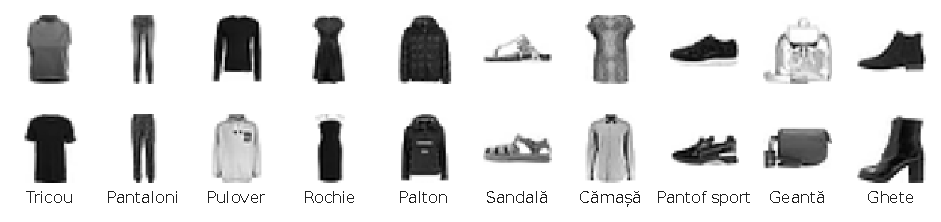
\includegraphics[width=\textwidth,height=0.280\textheight,keepaspectratio]{charts/ro/fmnist_samples.pdf}\end{center}\vspace{-3mm}
\chartsource{Sursa: Fashion-MNIST, Zalando Research (Xiao et al., 2017). Date: 60.000 de imagini de antrenare, 28 x 28 niveluri de gri.}
\vspace{0.5mm}
\begin{itemize}\setlength{\itemsep}{0pt}
  \item Fashion-MNIST: 50\,000 de imagini de antrenare, 10\,000 de validare și 10\,000 de test, din catalogul Zalando.
\end{itemize}
\par\vfill\manager{un magazin online etichetează zilnic mii de fotografii noi de produse
    \begin{itemize}\setlength{\itemsep}{0pt}
      \item Clasificatorul stabilește categoria, iar un operator verifică doar cazurile îndoielnice.
    \end{itemize}}\par\vspace{0.5mm}
\par\vfill\noindent{\scriptsize\color{FooterGray}(Xiao et al., 2017)}\hfill\qlink{NN\_L4\_fmnist\_samples}{Quantlets/L4/NN_L4_fmnist_samples}\par\vspace{0.5mm}
\end{frame}

\begin{frame}{Un strat dens pe pixeli irosește parametri și ignoră spațiul}
\footnotesize
\intuition{un MLP tratează pixelii (1,1) și (1,2) ca intrări fără legătură și are nevoie de cîte o pondere pentru fiecare pixel și fiecare unitate.}
\begin{columns}[T,onlytextwidth]
\begin{column}{0.53\textwidth}
\[ \mathbf h=\sigma(\mW\,\mathrm{vec}(\mathbf X)+\vb),\quad \mW\in\R^{m\times HWC} \]{\footnotesize\begin{itemize}\setlength{\itemsep}{0pt}
  \item \textbf{\txtwhere}
    \begin{itemize}\setlength{\itemsep}{0pt}
      \item $H,W$ înălțimea și lățimea
      \item $C$ numărul de canale
      \item $m$ unitățile ascunse
      \item O imagine color de $224\times224$ și $m=1000$ dau $224\cdot224\cdot3\cdot1000\approx1{,}5\cdot10^{8}$ ponderi numai în primul strat
    \end{itemize}
\end{itemize}\par}
\end{column}
\begin{column}{0.44\textwidth}
\begin{itemize}\setlength{\itemsep}{2pt}
  \item \textbf{Cele trei idei ale unei CNN}
    \begin{itemize}\setlength{\itemsep}{0pt}
      \item Conectivitate locală: o unitate vede doar o mică zonă
      \item Ponderi partajate: același filtru în toate pozițiile
      \item Echivarianță: o deplasare a intrării deplasează harta de trăsături, $f(T_{\delta}\mathbf X)=T_{\delta}f(\mathbf X)$
    \end{itemize}
  \item Pe datele noastre: MLP cu 235\,146 de parametri, CNN cu 140\,778, de 1{,}67 ori mai puțini.
\end{itemize}
\end{column}
\end{columns}
\par\vfill\manager{mai puțini parametri înseamnă mai puține date necesare pentru aceeași acuratețe, iar imaginile etichetate costă bani.}\par\vspace{0.5mm}
\par\vfill\noindent{\scriptsize\color{FooterGray}(LeCun et al., 1998; Bishop \& Bishop, 2024, cap.~10)}\par\vspace{0.5mm}
\end{frame}


\section{Stratul convoluțional}

\begin{frame}{Convoluția: același filtru mic glisează peste imagine}
\footnotesize
\intuition{fiecare ieșire este o sumă ponderată a unei vecinătăți de $k\times k$, cu aceleași ponderi peste tot.}
\begin{columns}[T,onlytextwidth]
\begin{column}{0.64\textwidth}
\[ Z_{o}(i,j)=b_o+\sum_{c=1}^{C_{\mathrm{in}}}\sum_{u=0}^{k-1}\sum_{v=0}^{k-1}K_{o,c}(u,v)\,X_c(i s+u-p,\;j s+v-p) \]{\footnotesize\begin{itemize}\setlength{\itemsep}{0pt}
  \item \textbf{\txtwhere}
    \begin{itemize}\setlength{\itemsep}{0pt}
      \item $X_c$ canalul de intrare $c$
      \item $K_{o,c}$ nucleul de $k\times k$ de la canalul $c$ la harta de ieșire $o$
      \item $b_o$ termenul liber
      \item $s$ pasul (stride)
      \item $p$ completarea cu zerouri (padding)
    \end{itemize}
\end{itemize}\par}
\end{column}
\begin{column}{0.33\textwidth}
\begin{itemize}\setlength{\itemsep}{2pt}
  \item Harta de trăsături a filtrului $o$: $A_o=\ReLU(Z_o)$, cu unitatea liniară rectificată (ReLU) $\max(0,z)$
    \begin{itemize}\setlength{\itemsep}{0pt}
      \item $K$ este învățat prin propagarea înapoi a erorii.
    \end{itemize}
\end{itemize}
\end{column}
\end{columns}
\par\vfill\manager{un filtru este un detector de tipare testat în fiecare poziție a imaginii, cu un cost de doar $k^2C_{\mathrm{in}}$ ponderi.}\par\vspace{0.5mm}
\par\vfill\noindent{\scriptsize\color{FooterGray}(Goodfellow et al., 2016, cap.~9)}\par\vspace{0.5mm}
\end{frame}

\begin{frame}{Filtrele construite de mînă găsesc deja drumurile și marginile parcelelor}
\small
\intuition{un nucleu Sobel răspunde acolo unde luminozitatea se schimbă pe o direcție; un nucleu de medie estompează imaginea.}
\vspace{-1mm}\[ K_x=\begin{psmallmatrix}-1&0&1\\-2&0&2\\-1&0&1\end{psmallmatrix},\quad K_y=K_x^{\top},\quad K_{\mathrm{mean}}=\tfrac19\mathbf 1_{3\times3} \]\vspace{-2mm}
\begin{center}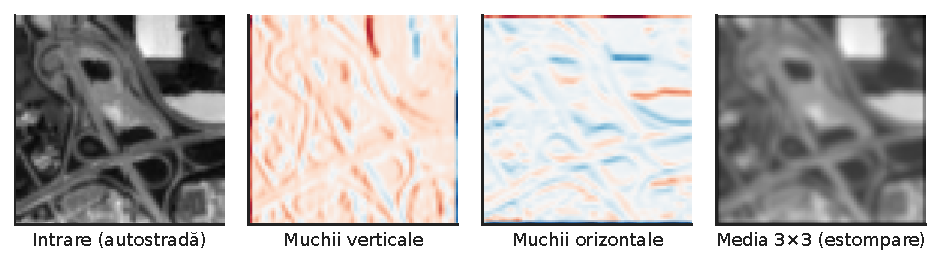
\includegraphics[width=\textwidth,height=0.360\textheight,keepaspectratio]{charts/ro/conv_edges.pdf}\end{center}\vspace{-3mm}
\chartsource{Sursa: EuroSAT, imagini Sentinel-2 (Helber et al., 2019). Date: o imagine Sentinel-2 de 64 x 64 (clasa Autostradă), niveluri de gri.}
\vspace{0.5mm}
\begin{itemize}\setlength{\itemsep}{0pt}
  \item Completarea $p=1$ păstrează dimensiunea de $64\times64$
    \begin{itemize}\setlength{\itemsep}{0pt}
      \item O CNN învață zeci de astfel de nuclee în fiecare strat, în loc să le fixeze.
    \end{itemize}
\end{itemize}
\par\vfill\noindent{\scriptsize\color{FooterGray}(calcul propriu)}\hfill\qlink{NN\_L4\_conv\_edges}{Quantlets/L4/NN_L4_conv_edges}\par\vspace{0.5mm}
\end{frame}

\begin{frame}{Dimensiunea ieșirii, completarea și pasul}
\footnotesize
\intuition{trei numere întregi decid cît de mare este fiecare hartă de trăsături.}
\begin{columns}[T,onlytextwidth]
\begin{column}{0.53\textwidth}
\[ H_{\mathrm{out}}=\Big\lfloor\frac{H_{\mathrm{in}}+2p-k}{s}\Big\rfloor+1 \]{\footnotesize\begin{itemize}\setlength{\itemsep}{0pt}
  \item \textbf{\txtwhere}
    \begin{itemize}\setlength{\itemsep}{0pt}
      \item $H_{\mathrm{in}}$ înălțimea intrării (aceeași formulă pentru lățime)
      \item $k$ dimensiunea nucleului
      \item $p$ completarea
      \item $s$ pasul
    \end{itemize}
\end{itemize}\par}
\end{column}
\begin{column}{0.44\textwidth}
\begin{itemize}\setlength{\itemsep}{2pt}
  \item \textbf{Exemple}, $H_{\mathrm{in}}=64$, $k=3$
    \begin{itemize}\setlength{\itemsep}{0pt}
      \item $p=1,s=1$: $H_{\mathrm{out}}=64$ (``same'')
      \item $p=0,s=1$: $H_{\mathrm{out}}=62$ (``valid'')
      \item $p=1,s=2$: $H_{\mathrm{out}}=32$ (subeșantionare)
    \end{itemize}
  \item Parametrii stratului: $(k^2C_{\mathrm{in}}+1)\,C_{\mathrm{out}}$, independenți de dimensiunea imaginii.
\end{itemize}
\end{column}
\end{columns}
\par\vfill\manager{aceeași rețea rulează pe imagini de orice dimensiune
    \begin{itemize}\setlength{\itemsep}{0pt}
      \item Crește doar costul în operații, $H_{\mathrm{out}}W_{\mathrm{out}}k^2C_{\mathrm{in}}C_{\mathrm{out}}$.
    \end{itemize}}\par\vspace{0.5mm}
\par\vfill\noindent{\scriptsize\color{FooterGray}(calcul propriu)}\par\vspace{0.5mm}
\end{frame}

\begin{frame}{Agregarea rezumă o vecinătate; agregarea globală rezumă imaginea}
\footnotesize
\intuition{agregarea prin maxim păstrează cel mai puternic răspuns din fiecare fereastră, micșorează harta și o face ușor invariantă la deplasări.}
\begin{columns}[T,onlytextwidth]
\begin{column}{0.53\textwidth}
\[ P_o(i,j)=\max_{0\le u,v<2}A_o(2i+u,2j+v) \]\vspace{-2mm}\[ g_o=\frac{1}{HW}\sum_{i,j}A_o(i,j) \]{\footnotesize\begin{itemize}\setlength{\itemsep}{0pt}
  \item \textbf{\txtwhere}
    \begin{itemize}\setlength{\itemsep}{0pt}
      \item $P_o$ agregarea prin maxim $2\times2$ cu pasul 2 (înjumătățește înălțimea și lățimea)
      \item $g_o$ agregarea prin medie globală (GAP), cîte un număr pentru fiecare canal
    \end{itemize}
\end{itemize}\par}
\end{column}
\begin{column}{0.44\textwidth}
\begin{itemize}\setlength{\itemsep}{2pt}
  \item CNN-ul nostru pentru Fashion-MNIST: hărți $28\times28\to14\times14\to7\times7$, apoi GAP dă 128 de numere, iar un strat liniar dă cele 10 scoruri ale claselor.
  \item Gradientul agregării prin maxim: trece doar prin poziția maximului din fiecare fereastră.
  \item GAP înlocuiește straturile dense mari (mii de ponderi) cu o medie (zero ponderi).
\end{itemize}
\end{column}
\end{columns}
\par\vfill\manager{GAP este motivul pentru care o CNN modernă are puțini parametri în partea finală și poate fi explicată cu hărți de activare ale claselor.}\par\vspace{0.5mm}
\par\vfill\noindent{\scriptsize\color{FooterGray}(Bishop \& Bishop, 2024, secț.~10.2)}\par\vspace{0.5mm}
\end{frame}

\begin{frame}{Adîncimea, agregarea și cîmpul receptiv}
\small
\intuition{cîmpul receptiv este zona din intrare care poate influența o unitate.}
\vspace{-1mm}\[ r_l=r_{l-1}+(k_l-1)\prod_{i<l}s_i,\qquad r_0=1 \]\vspace{-2mm}
\begin{center}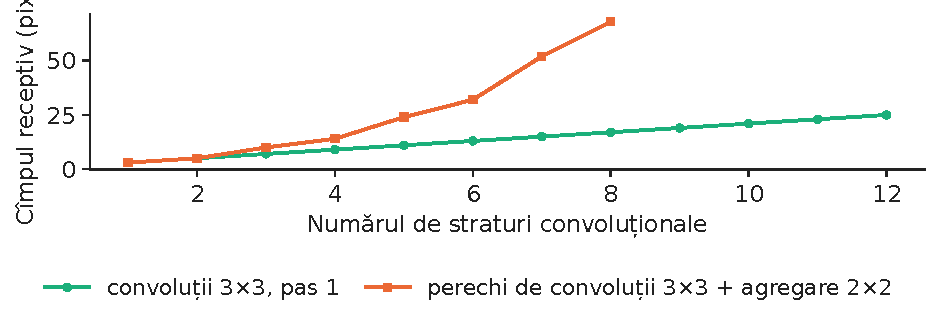
\includegraphics[width=\textwidth,height=0.360\textheight,keepaspectratio]{charts/ro/receptive_field.pdf}\end{center}\vspace{-3mm}
\chartsource{Sursa: calcul propriu din recurența cîmpului receptiv. Date: recurența cîmpului receptiv, fără date.}
\vspace{0.5mm}
\begin{itemize}\setlength{\itemsep}{0pt}
  \item Douăsprezece straturi $3\times3$ cu pasul 1 văd doar $25\times25$ pixeli
    \begin{itemize}\setlength{\itemsep}{0pt}
      \item Opt straturi cu agregare $2\times2$ după fiecare pereche văd $68\times68$.
    \end{itemize}
\end{itemize}
\par\vfill\noindent{\scriptsize\color{FooterGray}(calcul propriu)}\hfill\qlink{NN\_L4\_receptive\_field}{Quantlets/L4/NN_L4_receptive_field}\par\vspace{0.5mm}
\end{frame}

\begin{frame}{Propagarea înapoi printr-o convoluție este tot o convoluție}
\footnotesize
\intuition{pentru că nucleul este partajat, gradientul lui adună contribuțiile tuturor pozițiilor.}
\begin{columns}[T,onlytextwidth]
\begin{column}{0.53\textwidth}
\[ \frac{\partial\loss}{\partial K_{o,c}(u,v)}=\sum_{i,j}\delta_o(i,j)\,X_c(is+u-p,\,js+v-p) \]\vspace{-2mm}\[ \delta_o(i,j)=\frac{\partial\loss}{\partial Z_o(i,j)} \]{\footnotesize\begin{itemize}\setlength{\itemsep}{0pt}
  \item \textbf{\txtwhere}
    \begin{itemize}\setlength{\itemsep}{0pt}
      \item $\delta_o$ harta erorilor pentru ieșirea $o$, calculată prin propagarea înapoi din stratul superior
      \item Pentru $s=1$, $\partial\loss/\partial X_c=\sum_o \delta_o \star \mathrm{rot}_{180}(K_{o,c})$, o convoluție completă
    \end{itemize}
\end{itemize}\par}
\end{column}
\begin{column}{0.44\textwidth}
\begin{itemize}\setlength{\itemsep}{2pt}
  \item Partajarea ponderilor transformă milioane de gradienți specifici fiecărei poziții într-o singură sumă pentru fiecare pondere.
  \item În cod, diferențierea automată face totul: \texttt{loss.backward()} pe un \texttt{nn.Conv2d}.
  \item Derivarea completă este în anexă (convoluția ca produs de matrice).
\end{itemize}
\end{column}
\end{columns}
\par\vfill\manager{o trecere înainte și una înapoi costă aproximativ același număr de operații, deci timpul de antrenare crește odată cu costul trecerii înainte.}\par\vspace{0.5mm}
\par\vfill\noindent{\scriptsize\color{FooterGray}(Goodfellow et al., 2016, secț.~9.5)}\par\vspace{0.5mm}
\end{frame}

\begin{frame}{Normalizarea pe loturi menține fiecare canal pe aceeași scală}
\footnotesize
\intuition{fiecare canal este standardizat pe lot și pe poziții, apoi rescalat cu doi parametri învățați.}
\begin{columns}[T,onlytextwidth]
\begin{column}{0.53\textwidth}
\[ \hat a=\frac{a-\mu_{\mathcal B,o}}{\sqrt{\sigma^2_{\mathcal B,o}+\epsilon}},\qquad \mathrm{BN}(a)=\gamma_o\hat a+\beta_o \]{\footnotesize\begin{itemize}\setlength{\itemsep}{0pt}
  \item \textbf{\txtwhere}
    \begin{itemize}\setlength{\itemsep}{0pt}
      \item $\mu_{\mathcal B,o},\sigma^2_{\mathcal B,o}$ media și varianța canalului $o$ pe lotul $\mathcal B$ și pe toate pozițiile
      \item $\gamma_o,\beta_o$ învățați
      \item La testare, mediile mobile înlocuiesc statisticile lotului
    \end{itemize}
\end{itemize}\par}
\end{column}
\begin{column}{0.44\textwidth}
\begin{itemize}\setlength{\itemsep}{2pt}
  \item Toate rețelele din acest curs folosesc normalizarea pe loturi (BN) după fiecare convoluție: Conv $\to$ BN $\to$ ReLU.
  \item Permite rate de învățare mai mari
    \begin{itemize}\setlength{\itemsep}{0pt}
      \item Antrenările noastre pe CIFAR folosesc o programare one-cycle pînă la 0,1 (aleasă a priori).
    \end{itemize}
  \item Nu uitați \texttt{model.eval()} înainte de predicție: altfel BN folosește statisticile lotului de test.
\end{itemize}
\end{column}
\end{columns}
\par\vfill\manager{un model care merge bine în notebook, dar prost în producție, a uitat adesea modul eval sau scalarea intrărilor din antrenare.}\par\vspace{0.5mm}
\par\vfill\noindent{\scriptsize\color{FooterGray}(Ioffe \& Szegedy, 2015)}\par\vspace{0.5mm}
\end{frame}


\section{Studiu de caz: clasificarea fotografiilor de produse cu regresie softmax și CNN}

\begin{frame}{Protocolul experimental pentru cele trei modele}
\footnotesize
\begin{columns}[T,onlytextwidth]
\begin{column}{0.5\textwidth}
\begin{itemize}\setlength{\itemsep}{3pt}
  \item \textbf{Reper}: regresia softmax (logistică multinomială)
    \begin{itemize}\setlength{\itemsep}{0pt}
      \item $\hat{\mathbf p}=\softmax(\mW\mathrm{vec}(\mathbf X)+\vb)$, 7\,850 de parametri
    \end{itemize}
  \item \textbf{MLP}: 784--256--128--10, ReLU, dropout 0,2
    \begin{itemize}\setlength{\itemsep}{0pt}
      \item 235\,146 de parametri
    \end{itemize}
  \item \textbf{CNN}: 2 blocuri [Conv3$\times$3--BN--ReLU]$\times$2 + agregare maxim, Conv 128, GAP, liniar
    \begin{itemize}\setlength{\itemsep}{0pt}
      \item 140\,778 de parametri
    \end{itemize}
\end{itemize}
\end{column}
\begin{column}{0.47\textwidth}
\begin{itemize}\setlength{\itemsep}{3pt}
  \item \textbf{Aceeași antrenare pentru toate}
    \begin{itemize}\setlength{\itemsep}{0pt}
      \item AdamW, loturi de 128, 12 epoci, rată de învățare one-cycle
      \item Entropia încrucișată $\loss=-\frac1n\sum_i\log\hat p_{i,y_i}$
      \item Pixeli standardizați cu media de antrenare 0{,}2859 și abaterea standard 0{,}3530
    \end{itemize}
  \item \textbf{Comparație corectă}
    \begin{itemize}\setlength{\itemsep}{0pt}
      \item Oprire timpurie pe cele 10\,000 de imagini de validare
      \item 3 semințe pentru fiecare model; imaginile de test sînt folosite o singură dată
    \end{itemize}
\end{itemize}
\end{column}
\end{columns}
\par\vfill\manager{timpul total de antrenare al celor nouă rulări: 299 de secunde pe procesorul grafic al unui laptop.}\par\vspace{0.5mm}
\par\vfill\noindent{\scriptsize\color{FooterGray}(calcul propriu)}\hfill\tryit{\S3}\par\vspace{0.5mm}
\end{frame}

\begin{frame}{CNN învață mai repede și generalizează mai bine}
\small
\intuition{pierderea de validare scade cel mai mult pentru CNN; MLP se potrivește datelor de antrenare, dar nu mai progresează pe imagini noi.}
\begin{center}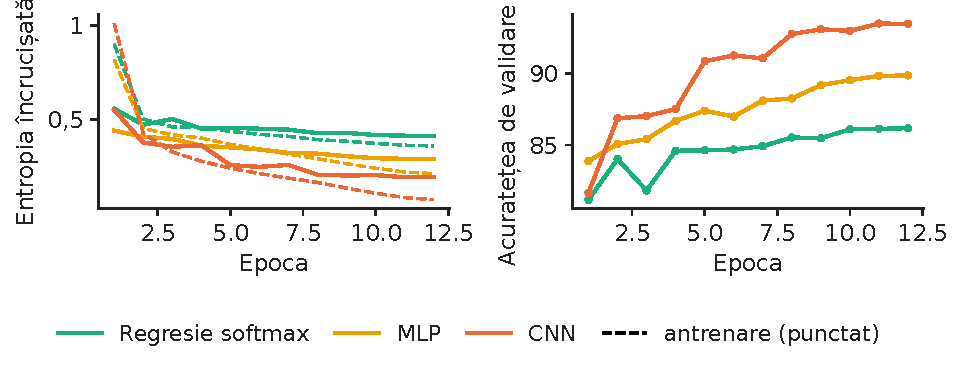
\includegraphics[width=\textwidth,height=0.500\textheight,keepaspectratio]{charts/ro/fmnist_curves.pdf}\end{center}\vspace{-3mm}
\chartsource{Sursa: Fashion-MNIST, Zalando Research (Xiao et al., 2017). Date: 50.000 de imagini de antrenare și 10.000 de validare; sămînța 20261108.}
\vspace{0.5mm}
\begin{itemize}\setlength{\itemsep}{0pt}
  \item Cea mai bună epocă pe validare (sămînța 20261108): CNN 11, MLP 12, softmax 12, din 12.
\end{itemize}
\par\vfill\noindent{\scriptsize\color{FooterGray}(calcul propriu)}\hfill\qlink{NN\_L4\_fmnist\_curves}{Quantlets/L4/NN_L4_fmnist_curves}\par\vspace{0.5mm}
\end{frame}

\begin{frame}{Acuratețea și numărul de parametri ai celor trei modele}
\small
\intuition{partajarea ponderilor aduce acuratețe și economisește parametri în același timp.}
\begin{center}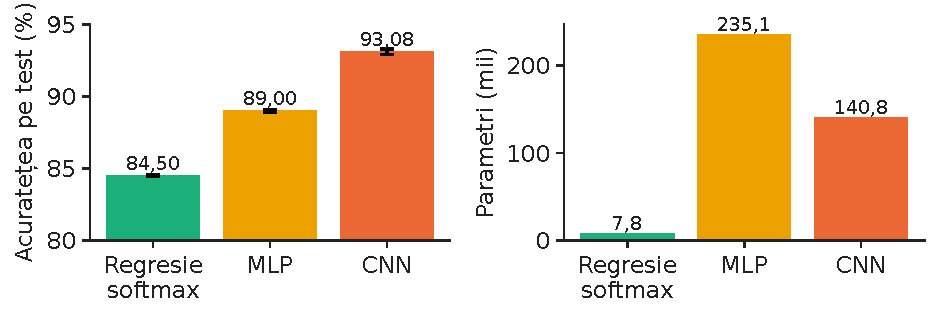
\includegraphics[width=\textwidth,height=0.420\textheight,keepaspectratio]{charts/ro/fmnist_compare.pdf}\end{center}\vspace{-3mm}
\chartsource{Sursa: Fashion-MNIST, Zalando Research (Xiao et al., 2017). Date: 10.000 de imagini de test; media și abaterea standard pe 3 semințe.}
\vspace{0.5mm}
\begin{itemize}\setlength{\itemsep}{0pt}
  \item Acuratețea pe test (medie $\pm$ abatere standard, 3 semințe): softmax 84{,}50\,$\pm$\,0{,}06\,\%, MLP 89{,}00\,$\pm$\,0{,}10\,\%, CNN 93{,}08\,$\pm$\,0{,}20\,\%.
  \item CNN elimină 37{,}1\,\% din erorile MLP, cu de 1{,}67 ori mai puțini parametri.
\end{itemize}
\par\vfill\noindent{\scriptsize\color{FooterGray}(calcul propriu)}\hfill\qlink{NN\_L4\_fmnist\_compare}{Quantlets/L4/NN_L4_fmnist_compare}\par\vspace{0.5mm}
\end{frame}

\begin{frame}{Testul McNemar pentru cîștigul de acuratețe pe aceleași imagini de test}
\footnotesize
\intuition{două clasificatoare evaluate pe aceleași imagini diferă doar prin imaginile pe care exact unul dintre ele le clasifică bine.}
\begin{columns}[T,onlytextwidth]
\begin{column}{0.53\textwidth}
\[ \chi^2=\frac{(|b-c|-1)^2}{b+c}\;\overset{H_0}{\sim}\;\chi^2_1 \]{\footnotesize\begin{itemize}\setlength{\itemsep}{0pt}
  \item \textbf{\txtwhere}
    \begin{itemize}\setlength{\itemsep}{0pt}
      \item $b$ imaginile corecte doar pentru CNN
      \item $c$ corecte doar pentru MLP
      \item $H_0$: ambele au aceeași rată de eroare
      \item Valoarea critică la 5\,\% este 3,84
    \end{itemize}
\end{itemize}\par}
\end{column}
\begin{column}{0.44\textwidth}
\begin{itemize}\setlength{\itemsep}{2pt}
  \item Sămînța 20261108: $b=614$, $c=226$, $\chi^2=178{,}3$: ipoteza nulă este respinsă.
  \item Pe cele 3 semințe, statistica $t$ pereche a diferenței de acuratețe este 31{,}38.
  \item Semințele măsoară zgomotul antrenării
    \begin{itemize}\setlength{\itemsep}{0pt}
      \item Testul McNemar măsoară zgomotul setului de test
      \item Raportați-le pe amîndouă.
    \end{itemize}
\end{itemize}
\end{column}
\end{columns}
\par\vfill\manager{înainte de a înlocui un model aflat în producție, arătați că avantajul rezistă unui test pe aceleași cazuri, nu doar o medie mai mare.}\par\vspace{0.5mm}
\par\vfill\noindent{\scriptsize\color{FooterGray}(McNemar, 1947)}\par\vspace{0.5mm}
\end{frame}

\begin{frame}{Matricea de confuzie: erori între produse cu forme asemănătoare}
\small
\intuition{cele mai multe greșeli apar între articolele pentru partea de sus a corpului, cu forme asemănătoare.}
\begin{center}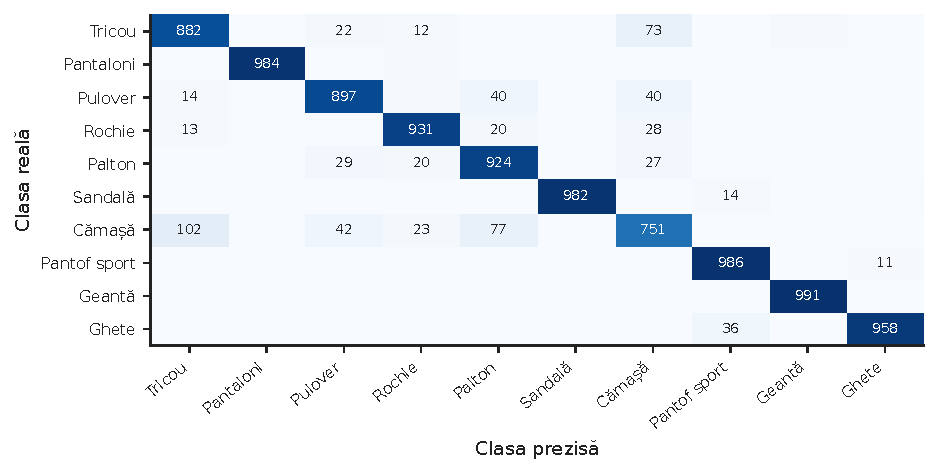
\includegraphics[width=\textwidth,height=0.393\textheight,keepaspectratio]{charts/ro/fmnist_confusion.pdf}\end{center}\vspace{-3mm}
\chartsource{Sursa: Fashion-MNIST, Zalando Research (Xiao et al., 2017). Date: 10.000 de imagini de test, CNN cu sămînța 20261108.}
\vspace{0.5mm}
\begin{itemize}\setlength{\itemsep}{0pt}
  \item Clasa cea mai slabă: Cămașă (sensibilitate 75{,}1\,\%)
    \begin{itemize}\setlength{\itemsep}{0pt}
      \item Cea mai mare confuzie: Cămașă clasificat drept Tricou, 102 de imagini.
    \end{itemize}
\end{itemize}
\par\vfill\manager{trimiteți la verificare umană doar fotografiile cu încredere scăzută din clasele slabe: costul erorilor scade acolo unde este cel mai mare.}\par\vspace{0.5mm}
\par\vfill\noindent{\scriptsize\color{FooterGray}(calcul propriu)}\hfill\qlink{NN\_L4\_fmnist\_confusion}{Quantlets/L4/NN_L4_fmnist_confusion}\par\vspace{0.5mm}
\end{frame}

\begin{frame}{Filtrele din primul strat detectează muchii și contraste}
\small
\intuition{nimeni nu i-a cerut rețelei să caute muchii; coborîrea pe gradient le-a găsit singură.}
\begin{center}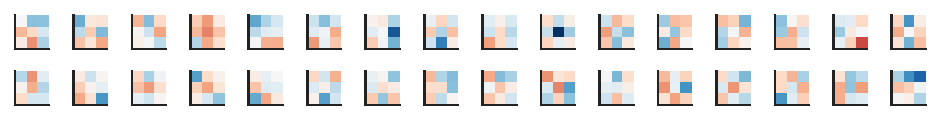
\includegraphics[width=\textwidth,height=0.200\textheight,keepaspectratio]{charts/ro/fmnist_filters.pdf}\end{center}\vspace{-3mm}
\chartsource{Sursa: Fashion-MNIST, Zalando Research (Xiao et al., 2017). Date: primul strat convoluțional al CNN (32 de filtre de 3 x 3), sămînța 20261108.}
\vspace{0.5mm}
\begin{itemize}\setlength{\itemsep}{0pt}
  \item Roșu = pondere pozitivă, albastru = negativă: multe nuclee sînt diferențe orientate, ca nucleele Sobel alese de mînă.
  \item Straturile mai adînci le combină în părți (gulere, tălpi, mînere) (Zeiler \& Fergus, 2014).
\end{itemize}
\par\vfill\noindent{\scriptsize\color{FooterGray}(calcul propriu; Zeiler \& Fergus, 2014)}\hfill\qlink{NN\_L4\_fmnist\_filters}{Quantlets/L4/NN_L4_fmnist_filters}\par\vspace{0.5mm}
\end{frame}

\begin{frame}{Hărțile de trăsături la adîncimi crescătoare}
\small
\intuition{hărțile timpurii păstrează conturul ghetei; cele adînci sînt mici, dar arată unde se află părțile informative.}
\begin{center}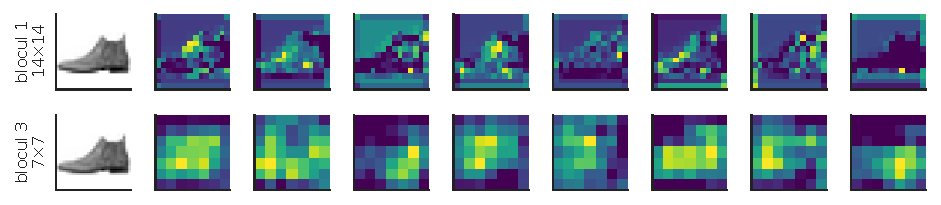
\includegraphics[width=\textwidth,height=0.360\textheight,keepaspectratio]{charts/ro/fmnist_featuremaps.pdf}\end{center}\vspace{-3mm}
\chartsource{Sursa: Fashion-MNIST, Zalando Research (Xiao et al., 2017). Date: o imagine de test (ghete); cele mai active 8 canale din fiecare bloc.}
\vspace{0.5mm}
\begin{itemize}\setlength{\itemsep}{0pt}
  \item Blocul 1: 32 de hărți de 14$\times$14
    \begin{itemize}\setlength{\itemsep}{0pt}
      \item Blocul 3: 128 de hărți de 7$\times$7, apoi mediate de GAP.
    \end{itemize}
\end{itemize}
\par\vfill\noindent{\scriptsize\color{FooterGray}(calcul propriu)}\hfill\qlink{NN\_L4\_fmnist\_featuremaps}{Quantlets/L4/NN_L4_fmnist_featuremaps}\par\vspace{0.5mm}
\end{frame}


\section{Arhitecturi: de la LeNet la ResNet}

\begin{frame}{Arhitecturi pentru recunoașterea imaginilor, 1998--2021}
\footnotesize
{\footnotesize\renewcommand{\arraystretch}{1.05}\setlength{\tabcolsep}{4pt}
\begin{tabular}{@{}p{0.17\textwidth}p{0.07\textwidth}p{0.68\textwidth}@{}}\toprule
Rețeaua & Anul & Ideea principală \\ \midrule
LeNet-5 & 1998 & convoluție + subeșantionare pentru cifre scrise de mînă (banc de probă MNIST); antrenată prin propagarea înapoi a erorii \\
AlexNet & 2012 & CNN adîncă pe ImageNet antrenată pe GPU; ReLU, dropout, augmentarea datelor \\
Visual Geometry Group (VGG) & 2015 & numai nuclee $3\times3$: două nuclee $3\times3$ suprapuse văd $5\times5$ cu $18C^2$ în loc de $25C^2$ ponderi \\
ResNet & 2016 & conexiuni reziduale $\mathbf y=\mathbf x+F(\mathbf x)$: rețelele cu peste 100 de straturi devin antrenabile \\
Transformer vizual & 2021 & fragmente de imagine tratate ca unități lexicale, cu atenție (cursul 7) \\
\bottomrule\end{tabular}}
\par\vspace{0.5mm}{\scriptsize \begin{itemize}\setlength{\itemsep}{0pt}
  \item ResNet-18, folosit mai jos pentru transferul învățării, are 11\,181\,642 de parametri (numărați de noi, cu un strat final de 10 clase).
\end{itemize}}
\par\vfill\noindent{\scriptsize\color{FooterGray}(LeCun et al., 1998; Krizhevsky et al., 2012; Simonyan \& Zisserman, 2015; He et al., 2016)}\par\vspace{0.5mm}
\end{frame}

\begin{frame}{Conexiunile reziduale și calea identității}
\footnotesize
\intuition{un bloc își adună ieșirea la intrare, astfel încît gradientul are mereu un drum direct înapoi.}
\begin{columns}[T,onlytextwidth]
\begin{column}{0.53\textwidth}
\[ \mathbf y=\ReLU\big(\mathbf x+F(\mathbf x;\mW)\big),\qquad \frac{\partial\loss}{\partial\mathbf x}=\frac{\partial\loss}{\partial\mathbf y}\Big(\mathbf I+\frac{\partial F}{\partial\mathbf x}\Big) \]{\footnotesize\begin{itemize}\setlength{\itemsep}{0pt}
  \item \textbf{\txtwhere}
    \begin{itemize}\setlength{\itemsep}{0pt}
      \item $F$ două straturi Conv--BN
      \item Cînd forma se schimbă, $\mathbf x$ trece printr-o convoluție $1\times1$ cu pasul 2
      \item Derivata este scrisă pentru suma dinaintea activării
    \end{itemize}
\end{itemize}\par}
\end{column}
\begin{column}{0.44\textwidth}
\begin{itemize}\setlength{\itemsep}{2pt}
  \item Rețelele adînci simple suferă de degradare: cele mai adînci au eroare de antrenare mai mare, o problemă de optimizare, nu de supraînvățare.
  \item Dacă cel mai bun bloc este identitatea, este suficient ca $F=0$.
  \item Pe CIFAR-10 (diapozitivul următor): aceleași 32 de straturi, cu și fără scurtătură.
\end{itemize}
\end{column}
\end{columns}
\par\vfill\manager{blocurile reziduale sînt alegerea implicită în toate modelele moderne de viziune și de limbaj, inclusiv în transformere.}\par\vspace{0.5mm}
\par\vfill\noindent{\scriptsize\color{FooterGray}(He et al., 2016)}\par\vspace{0.5mm}
\end{frame}

\begin{frame}{Efectele augmentării datelor și ale conexiunilor reziduale}
\small
\intuition{stînga: aceeași CNN pe fotografiile Canadian Institute for Advanced Research (CIFAR-10); dreapta: rețele de 32 de straturi care diferă doar prin scurtătură.}
\begin{center}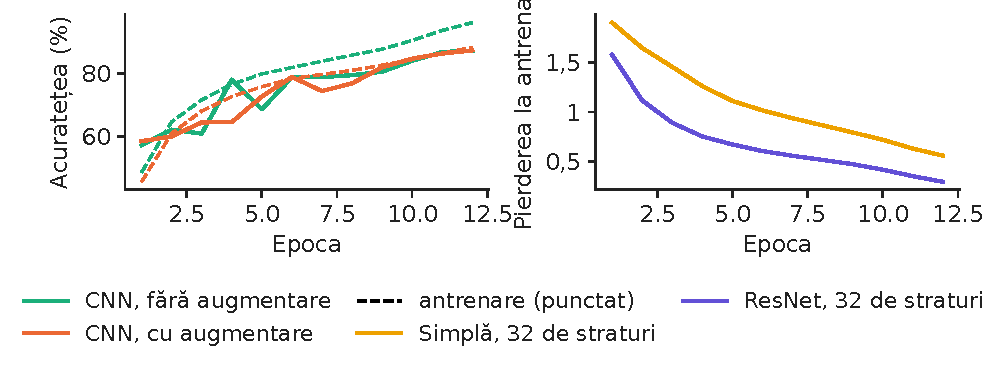
\includegraphics[width=\textwidth,height=0.420\textheight,keepaspectratio]{charts/ro/cifar_curves.pdf}\end{center}\vspace{-3mm}
\chartsource{Sursa: CIFAR-10 (Krizhevsky, 2009). Date: 45.000 de imagini de antrenare și 5.000 de validare; sămînța 20261108.}
\vspace{0.5mm}
\begin{itemize}\setlength{\itemsep}{0pt}
  \item Acuratețea pe test: CNN 86{,}56\,\% fără și 86{,}86\,\% cu augmentare (decalaj antrenare--validare 8{,}9 față de 0{,}9 puncte).
  \item Rețeaua simplă cu 32 de straturi 79{,}96\,\%, ResNet-32 87{,}81\,\%
    \begin{itemize}\setlength{\itemsep}{0pt}
      \item Pierderea finală la antrenare 0{,}557 față de 0{,}291.
    \end{itemize}
\end{itemize}
\par\vfill\noindent{\scriptsize\color{FooterGray}(calcul propriu)}\hfill\qlink{NN\_L4\_cifar\_curves}{Quantlets/L4/NN_L4_cifar_curves}\par\vspace{0.5mm}
\end{frame}

\begin{frame}{Augmentarea datelor ca informație a priori}
\footnotesize
\intuition{antrenăm pe transformări aleatoare care nu ar trebui să schimbe eticheta, adică mediem pierderea peste ele.}
\begin{columns}[T,onlytextwidth]
\begin{column}{0.53\textwidth}
\[ \min_{\btheta}\;\frac1n\sum_{i=1}^n\E_{T\sim\mathcal T}\Big[\ell\big(f_{\btheta}(T(\mathbf X_i)),y_i\big)\Big] \]{\footnotesize\begin{itemize}\setlength{\itemsep}{0pt}
  \item \textbf{\txtwhere}
    \begin{itemize}\setlength{\itemsep}{0pt}
      \item $\mathcal T$ mulțimea transformărilor care păstrează eticheta
      \item CIFAR-10: decupări aleatoare după o completare de 4 pixeli și oglindiri orizontale
      \item EuroSAT: oglindiri și rotații cu $90^\circ$
    \end{itemize}
\end{itemize}\par}
\end{column}
\begin{column}{0.44\textwidth}
\begin{itemize}\setlength{\itemsep}{2pt}
  \item Cîștigul pe CIFAR-10, pentru aceeași rețea și același buget: \ensuremath{+}0{,}30 puncte procentuale de acuratețe pe test.
  \item Alegeți $\mathcal T$ după domeniu: o cifră 6 oglindită nu mai este 6, dar o imagine satelitară nu are ``sus''.
  \item Sensibilitatea pe clase a ResNet-32: cea mai bună automobil 95{,}7\,\%, cea mai slabă pisică 71{,}9\,\%.
\end{itemize}
\end{column}
\end{columns}
\par\vfill\manager{augmentarea înseamnă date suplimentare gratuite
    \begin{itemize}\setlength{\itemsep}{0pt}
      \item Este prima pîrghie de folosit înainte de a cumpăra mai multe etichete.
    \end{itemize}}\par\vspace{0.5mm}
\par\vfill\noindent{\scriptsize\color{FooterGray}(calcul propriu)}\par\vspace{0.5mm}
\end{frame}


\section{Transferul învățării: utilizarea terenului din imagini satelitare}

\begin{frame}{Imagini satelitare: utilizarea terenului pentru creditori, asigurători și investitori}
\small
\intuition{zece clase de utilizare a terenului din imagini Sentinel-2 ale unor țări din Uniunea Europeană (UE); întrebarea este cu cît de puține etichete ne descurcăm.}
\vspace{-1mm}\[ \mathbf X\in[0,1]^{64\times64\times3},\qquad y\in\{\text{culturi},\dots,\text{mare/lac}\} \]\vspace{-2mm}
\begin{center}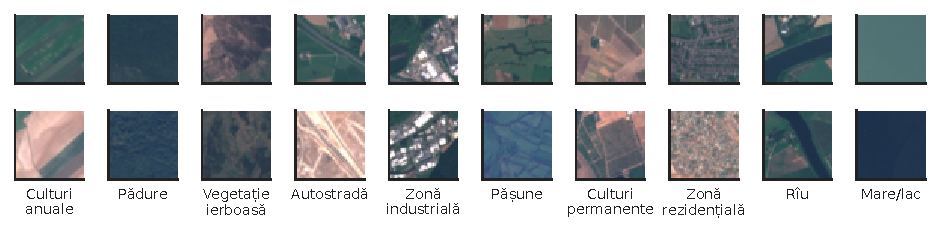
\includegraphics[width=\textwidth,height=0.291\textheight,keepaspectratio]{charts/ro/eurosat_samples.pdf}\end{center}\vspace{-3mm}
\chartsource{Sursa: EuroSAT, imagini Sentinel-2 (Helber et al., 2019). Date: 27.000 de imagini de 64 x 64 pixeli, 10 clase.}
\vspace{0.5mm}
\begin{itemize}\setlength{\itemsep}{0pt}
  \item 27\,000 de imagini roșu, verde, albastru (RGB) de $64\times64$ pixeli
    \begin{itemize}\setlength{\itemsep}{0pt}
      \item Între 2\,000 și 3\,000 pe clasă.
    \end{itemize}
\end{itemize}
\par\vfill\manager{un creditor agricol verifică dacă un împrumut finanțează culturi
    \begin{itemize}\setlength{\itemsep}{0pt}
      \item Un asigurător cartografiază zonele rezidențiale expuse inundațiilor.
    \end{itemize}}\par\vspace{0.5mm}
\par\vfill\noindent{\scriptsize\color{FooterGray}(Helber et al., 2019)}\hfill\qlink{NN\_L4\_eurosat\_samples}{Quantlets/L4/NN_L4_eurosat_samples}\par\vspace{0.5mm}
\end{frame}

\begin{frame}{Transferul învățării: trăsături învățate pe un milion de fotografii}
\footnotesize
\intuition{primele straturi ale unei rețele antrenate pe ImageNet detectează muchii și texturi utile pentru orice imagine.}
\begin{columns}[T,onlytextwidth]
\begin{column}{0.53\textwidth}
\[ f_{\btheta}(\mathbf X)=g_{\boldsymbol\psi}\big(\phi_{\boldsymbol\omega}(\mathbf X)\big),\quad \boldsymbol\omega^{(0)}=\boldsymbol\omega_{\mathrm{ImageNet}} \]{\footnotesize\begin{itemize}\setlength{\itemsep}{0pt}
  \item \textbf{\txtwhere}
    \begin{itemize}\setlength{\itemsep}{0pt}
      \item $\phi_{\boldsymbol\omega}$ corpul convoluțional (512 trăsături după GAP)
      \item $g_{\boldsymbol\psi}$ un nou strat final liniar cu 10 ieșiri
    \end{itemize}
\end{itemize}\par}
\end{column}
\begin{column}{0.44\textwidth}
\begin{itemize}\setlength{\itemsep}{2pt}
  \item \textbf{Extragerea trăsăturilor}
    \begin{itemize}\setlength{\itemsep}{0pt}
      \item $\boldsymbol\omega$ înghețat; se estimează doar $\boldsymbol\psi$ (aici o regresie logistică, cu $C$ ales pe validare)
    \end{itemize}
  \item \textbf{Ajustarea fină}
    \begin{itemize}\setlength{\itemsep}{0pt}
      \item Toate ponderile sînt antrenate, cu rată de învățare mai mică pentru corp ($3\cdot10^{-4}$) decît pentru stratul final ($3\cdot10^{-3}$), alese a priori
    \end{itemize}
  \item \textbf{De la zero}
    \begin{itemize}\setlength{\itemsep}{0pt}
      \item O CNN cu 4 blocuri, 1\,176\,746 de parametri, inițializare aleatoare
    \end{itemize}
\end{itemize}
\end{column}
\end{columns}
\par\vfill\manager{extragerea trăsăturilor este cea mai ieftină: o singură trecere prin imagini și o regresie logistică.}\par\vspace{0.5mm}
\par\vfill\noindent{\scriptsize\color{FooterGray}(Yosinski et al., 2014)}\par\vspace{0.5mm}
\end{frame}

\begin{frame}{Protocolul experimental pentru cele trei strategii de transfer}
\footnotesize
\begin{columns}[T,onlytextwidth]
\begin{column}{0.5\textwidth}
\begin{itemize}\setlength{\itemsep}{3pt}
  \item \textbf{Împărțirea}, stratificată pe clase
    \begin{itemize}\setlength{\itemsep}{0pt}
      \item 16\,200 de imagini de antrenare / 5\,400 de validare / 5\,400 de test
    \end{itemize}
  \item \textbf{Intrarea}
    \begin{itemize}\setlength{\itemsep}{0pt}
      \item Imaginile sînt redimensionate la $112\times112$ pentru ResNet-18 și scalate cu media și abaterea standard ImageNet ale fiecărui canal
      \item $\tilde x_c=(x_c-\mu_c)/s_c$
    \end{itemize}
\end{itemize}
\end{column}
\begin{column}{0.47\textwidth}
\begin{itemize}\setlength{\itemsep}{3pt}
  \item \textbf{Antrenarea}
    \begin{itemize}\setlength{\itemsep}{0pt}
      \item AdamW, loturi de 64, programare one-cycle; oglindiri și rotații cu $90^\circ$
      \item De la zero 18 epoci; ajustare fină 6 epoci
      \item Se păstrează modelul cu cea mai bună acuratețe de validare
    \end{itemize}
  \item \textbf{Costul}
    \begin{itemize}\setlength{\itemsep}{0pt}
      \item 1225 de secunde pentru cele trei rulări principale, pe procesorul grafic al unui laptop
    \end{itemize}
\end{itemize}
\end{column}
\end{columns}
\par\vfill\manager{fixarea imaginilor de test înaintea oricărei modelări face comparabile cele trei strategii.}\par\vspace{0.5mm}
\par\vfill\noindent{\scriptsize\color{FooterGray}(calcul propriu)}\hfill\tryit{\S5}\par\vspace{0.5mm}
\end{frame}

\begin{frame}{Ajustarea fină este cea mai precisă, iar transferul contează cel mai mult cînd etichetele sînt puține}
\small
\intuition{stînga: învățarea cu toate etichetele; dreapta: acuratețea pe test cînd sînt disponibile doar $n$ imagini etichetate pe clasă.}
\begin{center}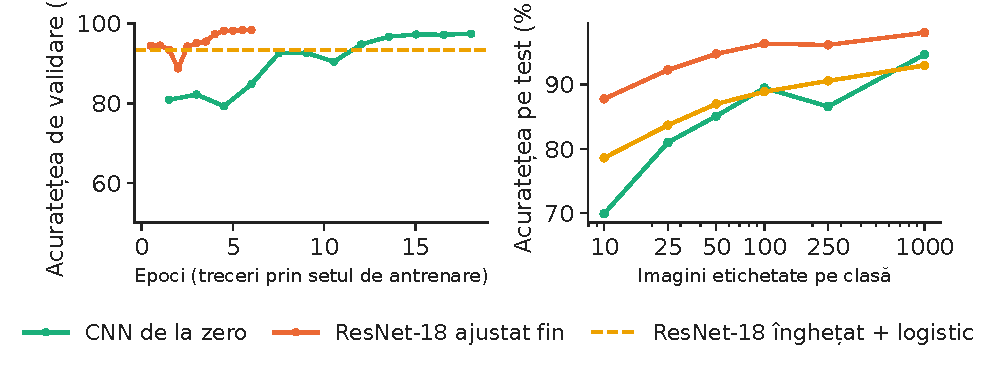
\includegraphics[width=\textwidth,height=0.333\textheight,keepaspectratio]{charts/ro/transfer_curves.pdf}\end{center}\vspace{-3mm}
\chartsource{Sursa: EuroSAT, imagini Sentinel-2 (Helber et al., 2019). Date: 16.200 de imagini de antrenare, 5.400 de validare, 5.400 de test; dreapta: media pe 2 semințe.}
\vspace{0.5mm}
\begin{itemize}\setlength{\itemsep}{0pt}
  \item Acuratețea pe test, cu toate etichetele: de la zero 97{,}78\,\%, înghețat + logistic 93{,}48\,\%, ajustat fin 98{,}76\,\%.
  \item Cu 10 imagini pe clasă: de la zero 69{,}9\,\%, înghețat 78{,}6\,\%, ajustat fin 87{,}8\,\%.
\end{itemize}
\par\vfill\noindent{\scriptsize\color{FooterGray}(calcul propriu)}\hfill\qlink{NN\_L4\_transfer\_curves}{Quantlets/L4/NN_L4_transfer_curves}\par\vspace{0.5mm}
\end{frame}

\begin{frame}{Bugetul de etichete și economia obținută prin transferul învățării}
\footnotesize
\begin{columns}[T,onlytextwidth]
\begin{column}{0.47\textwidth}
{\footnotesize\renewcommand{\arraystretch}{1.05}\setlength{\tabcolsep}{4pt}
\begin{tabular}{@{}rrrr@{}}\toprule
Imagini/clasă & De la zero & Înghețat & Ajustat fin \\ \midrule
10 & 69{,}9 & 78{,}6 & 87{,}8 \\
25 & 81{,}0 & 83{,}7 & 92{,}3 \\
50 & 85{,}1 & 87{,}0 & 94{,}8 \\
100 & 89{,}5 & 88{,}9 & 96{,}4 \\
250 & 86{,}6 & 90{,}6 & 96{,}2 \\
1000 & 94{,}7 & 93{,}0 & 98{,}1 \\
\bottomrule\end{tabular}}
\par\vspace{0.5mm}{\scriptsize \begin{itemize}\setlength{\itemsep}{0pt}
  \item Acuratețea pe test (\%), media a 2 extrageri aleatoare ale imaginilor etichetate; aceleași 5.400 de imagini de test.
\end{itemize}}
\end{column}
\begin{column}{0.5\textwidth}
\begin{itemize}\setlength{\itemsep}{4pt}
  \item Cu doar 100 de imagini etichetate în total, rețeaua preantrenată depășește clar o CNN antrenată de la zero pe aceleași etichete.
  \item CNN-ul de la zero are nevoie de întregul buget pentru a se apropia de rețeaua ajustată fin.
  \item Rularea întregului tabel a durat 1857 de secunde.
\end{itemize}
\end{column}
\end{columns}
\par\vfill\manager{etichetarea unei imagini costă un minut de lucru al unui expert
    \begin{itemize}\setlength{\itemsep}{0pt}
      \item Transferul învățării transformă săptămîni de etichetare într-o după-amiază.
    \end{itemize}}\par\vspace{0.5mm}
\par\vfill\noindent{\scriptsize\color{FooterGray}(calcul propriu)}\par\vspace{0.5mm}
\end{frame}

\begin{frame}{Erorile rămase: culturi anuale față de culturi permanente}
\small
\intuition{rețeaua ajustată fin confundă clase care arată la fel din spațiu.}
\begin{center}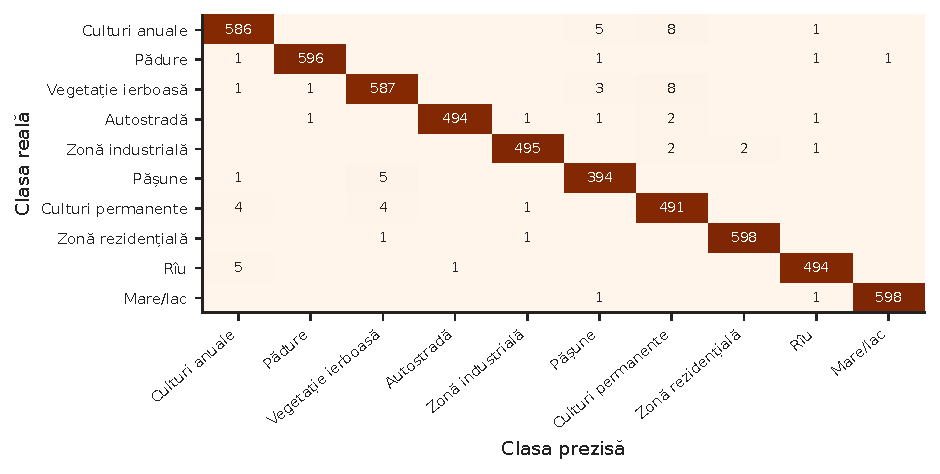
\includegraphics[width=\textwidth,height=0.500\textheight,keepaspectratio]{charts/ro/eurosat_confusion.pdf}\end{center}\vspace{-3mm}
\chartsource{Sursa: EuroSAT, imagini Sentinel-2 (Helber et al., 2019). Date: 5.400 de imagini de test, ResNet-18 ajustat fin, sămînța 20261108.}
\vspace{0.5mm}
\begin{itemize}\setlength{\itemsep}{0pt}
  \item 67 de erori la 5\,400 de imagini
    \begin{itemize}\setlength{\itemsep}{0pt}
      \item Cea mai mare: Culturi anuale clasificat drept Culturi permanente (8)
      \item Macro-F1 98{,}72\,\%.
    \end{itemize}
\end{itemize}
\par\vfill\noindent{\scriptsize\color{FooterGray}(calcul propriu)}\hfill\qlink{NN\_L4\_eurosat\_confusion}{Quantlets/L4/NN_L4_eurosat_confusion}\par\vspace{0.5mm}
\end{frame}

\begin{frame}{Grad-CAM: regiunile imaginii care determină clasificarea}
\footnotesize
\intuition{ponderăm fiecare hartă de trăsături după cît reacționează scorul clasei la ea, adunăm și păstrăm partea pozitivă.}
\begin{columns}[T,onlytextwidth]
\begin{column}{0.46\textwidth}
\[ \alpha^{c}_o=\frac{1}{HW}\sum_{i,j}\frac{\partial z_c}{\partial A_o(i,j)} \]\vspace{-2mm}\[ M^{c}=\ReLU\Big(\sum_o\alpha^{c}_oA_o\Big) \]{\footnotesize\begin{itemize}\setlength{\itemsep}{0pt}
  \item \textbf{\txtwhere}
    \begin{itemize}\setlength{\itemsep}{0pt}
      \item $z_c$ scorul (logitul) clasei $c$
      \item $A_o$ harta de trăsături $o$ din stratul ales
      \item $M^c$ harta de activare a clasei (CAM), mărită la dimensiunea imaginii
    \end{itemize}
\end{itemize}\par}
\end{column}
\begin{column}{0.51\textwidth}
\begin{center}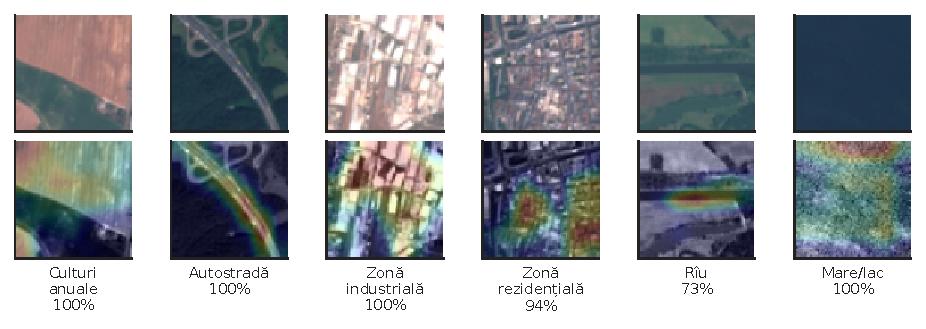
\includegraphics[width=\textwidth,height=0.550\textheight,keepaspectratio]{charts/ro/gradcam.pdf}\end{center}\vspace{-3mm}
\chartsource{Sursa: EuroSAT, imagini Sentinel-2 (Helber et al., 2019). Date: șase imagini de test; Grad-CAM pe hărțile de 7 x 7 ale blocului 3 din ResNet-18 ajustat fin.}
\end{column}
\end{columns}
\par\vfill\manager{un auditor poate verifica dacă ``zonă industrială'' este decisă de acoperișuri, nu de un nor sau de un artefact de margine.}\par\vspace{0.5mm}
\par\vfill\noindent{\scriptsize\color{FooterGray}(Selvaraju et al., 2017; calcul propriu)}\hfill\qlink{NN\_L4\_gradcam}{Quantlets/L4/NN_L4_gradcam}\par\vspace{0.5mm}
\end{frame}

\begin{frame}{Ponderile utilizării terenului estimate din imagini satelitare}
\footnotesize
\intuition{o întrebare de portofoliu privește ponderi și totaluri, deci erorile care se compensează contează mai puțin decît cele care nu se compensează.}
\begin{columns}[T,onlytextwidth]
\begin{column}{0.53\textwidth}
\[ \hat\pi_k=\frac1n\sum_{i=1}^n\mathbf 1\{\hat y_i=k\},\qquad \E[\hat\pi_k]=\sum_j\pi_j\,P(\hat y=k\mid y=j) \]{\footnotesize\begin{itemize}\setlength{\itemsep}{0pt}
  \item \textbf{\txtwhere}
    \begin{itemize}\setlength{\itemsep}{0pt}
      \item $\pi_k$ ponderea reală a clasei $k$ într-o regiune
      \item $P(\hat y=k\mid y=j)$ matricea de confuzie, estimată pe imaginile de test
    \end{itemize}
\end{itemize}\par}
\end{column}
\begin{column}{0.44\textwidth}
\begin{itemize}\setlength{\itemsep}{2pt}
  \item Imaginile de test: ponderea culturilor (anuale + permanente) este 20{,}37\,\% în realitate și 20{,}54\,\% prezisă.
  \item Cea mai mare eroare a ponderii oricărei clase: 0{,}20 puncte procentuale.
  \item Inversarea matricei de confuzie corectează ponderile atunci cînd ratele de eroare sînt stabile (schimbarea domeniului strică acest lucru).
\end{itemize}
\end{column}
\end{columns}
\par\vfill\manager{pentru un asigurător sau un creditor agricol, rezultatul este ponderea hectarelor pe regiune, cu o marjă de eroare, nu o etichetă pentru fiecare imagine.}\par\vspace{0.5mm}
\par\vfill\noindent{\scriptsize\color{FooterGray}(calcul propriu)}\par\vspace{0.5mm}
\end{frame}

\begin{frame}{Avantajele și riscurile transferului învățării}
\footnotesize
\begin{columns}[T,onlytextwidth]
\begin{column}{0.49\textwidth}
\begin{itemize}\setlength{\itemsep}{4pt}
  \item \textbf{Ajută cel mai mult}
    \begin{itemize}\setlength{\itemsep}{0pt}
      \item Cînd sînt puține etichete (panoul din dreapta al graficului de transfer)
      \item Cînd domeniul sursă are statistici de nivel jos similare (muchii, texturi)
      \item Cînd puterea de calcul este limitată: trăsăturile înghețate costă o singură trecere înainte
    \end{itemize}
\end{itemize}
\end{column}
\begin{column}{0.48\textwidth}
\begin{itemize}\setlength{\itemsep}{4pt}
  \item \textbf{Poate induce în eroare}
    \begin{itemize}\setlength{\itemsep}{0pt}
      \item Schimbarea domeniului: alt anotimp, alt senzor, altă țară decît imaginile de antrenare
      \item Indicii false învățate din sursă (filigrane, margini)
      \item Setul de test trebuie să provină din populația în care va fi folosit modelul
    \end{itemize}
\end{itemize}
\end{column}
\end{columns}
\par\vfill\manager{înainte de utilizare, etichetați un mic eșantion din regiunea țintă și măsurați din nou
    \begin{itemize}\setlength{\itemsep}{0pt}
      \item Modelul ajustat fin se actualizează ieftin.
    \end{itemize}}\par\vspace{0.5mm}
\par\vfill\noindent{\scriptsize\color{FooterGray}(Yosinski et al., 2014; Helber et al., 2019)}\par\vspace{0.5mm}
\end{frame}

\begin{frame}{Convoluții pentru secvențe și grafice}
\footnotesize
\intuition{o convoluție unidimensională glisează în timp, la fel cum una bidimensională glisează în spațiu.}
\begin{columns}[T,onlytextwidth]
\begin{column}{0.53\textwidth}
\[ z_t=b+\sum_{c}\sum_{u=0}^{k-1}K_c(u)\,x_{c,\,t-u} \]{\footnotesize\begin{itemize}\setlength{\itemsep}{0pt}
  \item \textbf{\txtwhere}
    \begin{itemize}\setlength{\itemsep}{0pt}
      \item $x_{c,t}$ seria de intrare $c$ la momentul $t$ (randamente, volum, consum)
      \item Cauzală: doar valori trecute
    \end{itemize}
\end{itemize}\par}
\end{column}
\begin{column}{0.44\textwidth}
\begin{itemize}\setlength{\itemsep}{2pt}
  \item O CNN unidimensională este un set învățat de filtre de tip medie mobilă
    \begin{itemize}\setlength{\itemsep}{0pt}
      \item Cursul 5 o compară cu rețelele recurente.
    \end{itemize}
  \item Graficele piețelor pot fi citite ca imagini de un model viziune--limbaj (VLM): cercetarea grupului nostru, în secțiunea următoare.
  \item Aceleași reguli: date reale, împărțire în ordine cronologică, întîi un model de referință simplu.
\end{itemize}
\end{column}
\end{columns}
\par\vfill\manager{un departament de risc poate examina zilnic sute de grafice cu un model, iar analistul se ocupă doar de cele semnalate.}\par\vspace{0.5mm}
\par\vfill\noindent{\scriptsize\color{FooterGray}(Bishop \& Bishop, 2024, cap.~10)}\par\vspace{0.5mm}
\end{frame}

\section*{Recapitulare}

\begin{frame}{Test 1: dimensiunea ieșirii}
\small
\begin{itemize}
  \item O imagine de $64\times64$ trece printr-o convoluție $3\times3$ cu completare 1 și pasul 2
    \begin{itemize}\setlength{\itemsep}{0pt}
      \item Cît de mare este harta de ieșire?
    \end{itemize}
\end{itemize}
\vspace{2mm}
\begin{exampleblock}{R\u{a}spuns}
\begin{itemize}
  \item $\lfloor(64+2-3)/2\rfloor+1=32$, deci $32\times32$.
\end{itemize}
\end{exampleblock}
\end{frame}

\begin{frame}{Test 2: parametrii}
\small
\begin{itemize}
  \item De ce depășește CNN-ul nostru MLP pe Fashion-MNIST, deși are mai puțini parametri?
\end{itemize}
\vspace{2mm}
\begin{exampleblock}{R\u{a}spuns}
\begin{itemize}
  \item Partajarea ponderilor și conectivitatea locală codifică structura imaginilor
    \begin{itemize}\setlength{\itemsep}{0pt}
      \item CNN atinge 93{,}08\,\% cu 140\,778 de parametri, față de 89{,}00\,\% cu 235\,146.
    \end{itemize}
\end{itemize}
\end{exampleblock}
\end{frame}

\begin{frame}{Test 3: adîncimea}
\small
\begin{itemize}
  \item O rețea simplă de 32 de straturi are o pierdere la antrenare mai mare decît una reziduală de aceeași adîncime
    \begin{itemize}\setlength{\itemsep}{0pt}
      \item Este supraînvățare?
    \end{itemize}
\end{itemize}
\vspace{2mm}
\begin{exampleblock}{R\u{a}spuns}
\begin{itemize}
  \item Nu: supraînvățarea scade pierderea la antrenare
    \begin{itemize}\setlength{\itemsep}{0pt}
      \item Aceasta este problema degradării (0{,}557 față de 0{,}291), rezolvată de scurtătura identitate.
    \end{itemize}
\end{itemize}
\end{exampleblock}
\end{frame}

\begin{frame}{Test 4: un buget de etichete}
\small
\begin{itemize}
  \item Puteți eticheta în total doar 100 de imagini satelitare
    \begin{itemize}\setlength{\itemsep}{0pt}
      \item Ce strategie alegeți?
    \end{itemize}
\end{itemize}
\vspace{2mm}
\begin{exampleblock}{R\u{a}spuns}
\begin{itemize}
  \item O rețea preantrenată: cu 10 imagini pe clasă, ajustarea fină dă 87{,}8\,\%, iar trăsăturile înghețate 78{,}6\,\%, față de 69{,}9\,\% de la zero.
\end{itemize}
\end{exampleblock}
\end{frame}

\begin{frame}{Test 5: explicația}
\small
\begin{itemize}
  \item Harta Grad-CAM a unei imagini ``zonă industrială'' evidențiază un nor
    \begin{itemize}\setlength{\itemsep}{0pt}
      \item Ce faceți?
    \end{itemize}
\end{itemize}
\vspace{2mm}
\begin{exampleblock}{R\u{a}spuns}
\begin{itemize}
  \item O tratați ca pe un semnal de indiciu fals: verificați imagini asemănătoare, adăugați exemple cu nori sau o mască de nori și testați din nou pe regiunea țintă.
\end{itemize}
\end{exampleblock}
\end{frame}

\begin{frame}{Recapitulare}
\small
\vspace{-2mm}\begin{multicols}{2}\scriptsize\tableofcontents\end{multicols}
\begin{itemize}\setlength{\itemsep}{1pt}
  \item O convoluție este un filtru local partajat
    \begin{itemize}\setlength{\itemsep}{0pt}
      \item Completarea, pasul și agregarea stabilesc dimensiunea hărții, iar adîncimea și agregarea cîmpul receptiv.
    \end{itemize}
  \item Pe imagini reale, CNN depășește MLP cu mai puțini parametri
    \begin{itemize}\setlength{\itemsep}{0pt}
      \item Blocurile reziduale fac adîncimea antrenabilă
      \item Augmentarea înseamnă date gratuite.
    \end{itemize}
  \item Transferul învățării cîștigă atunci cînd etichetele sînt rare
    \begin{itemize}\setlength{\itemsep}{0pt}
      \item Urmează secvențele și rețelele recurente (cursul 5).
    \end{itemize}
\end{itemize}
\end{frame}

\begin{frame}{Cercetări ale grupului nostru: modele de viziune în finanțe}
\footnotesize
\begin{itemize}\setlength{\itemsep}{4pt}
  \item \textbf{Un cadru multimodal viziune--limbaj pentru detectarea anomaliilor financiare} (Jheng, Pele, Tak \& Găman, 2026, PICBE), premiul Best Paper la International Conference on Business Excellence (ICBE) 2026
    \begin{itemize}\setlength{\itemsep}{0pt}
      \item Indicatorii de piață sînt proiectați într-o imagine standardizată, cu mai multe panouri; clasificarea regimurilor de piață devine o problemă de recunoaștere vizuală
      \item Model viziune--limbaj folosit fără antrenare suplimentară (GPT-4.1, transformer generativ preantrenat), cu etichete din cuantile glisante și justificări structurate în limbaj natural
      \item Teste în afara eșantionului pe S\&P 500: detectarea anomaliilor sistemice cu o fidelitate promițătoare și cu explicații interpretabile
    \end{itemize}
  \item \textbf{Quantlet: platforma de cunoștințe pentru fragmente de cod} (Găman, Winkel, Zuo, Härdle \& Pele, 2026, Computational Statistics)
    \begin{itemize}\setlength{\itemsep}{0pt}
      \item Platforma pe care fiecare grafic din acest curs este publicat ca Quantlet reproductibil
    \end{itemize}
\end{itemize}
\par\vspace{0.5mm}{\scriptsize \begin{itemize}\setlength{\itemsep}{0pt}
  \item Rezultatele de pe acest diapozitiv sînt cele raportate în lucrări; celelalte cifre din curs provin din calculele noastre.
\end{itemize}}
\par\vfill\noindent{\scriptsize\color{FooterGray}(Academia de Studii Economice din București; Academia Română, Institutul de Prognoză Economică)}\par\vspace{0.5mm}
\end{frame}

\begin{frame}{Lecturi și resurse suplimentare}
\small
\begin{columns}[T,onlytextwidth]
\begin{column}{0.52\textwidth}
\begin{itemize}\setlength{\itemsep}{4pt}
  \item \textbf{Bishop \& Bishop (2024)}, cap.~10: rețele convoluționale, cu derivările din acest curs.
  \item \textbf{Goodfellow, Bengio \& Courville (2016)}, cap.~9: convoluție, agregare, variante.
  \item \textbf{He et al. (2016)}: articolul ResNet, scurt și ușor de citit.
\end{itemize}
\end{column}
\begin{column}{0.45\textwidth}
\begin{itemize}\setlength{\itemsep}{4pt}
  \item \textbf{Acest curs}: cod, date, notebook-uri Jupyter --- \href{https://github.com/danpele/NEURAL_BIZ}{github.com/danpele/NEURAL\_BIZ}.
  \item \textbf{Exercițiu practic}: notebook-ul reproduce graficele acestui curs --- \href{\nnrepo/\nnnb}{notebooks/}.
  \item \textbf{Seminarul 4}: transferul învățării pe EuroSAT, cu propriul buget de etichete.
\end{itemize}
\end{column}
\end{columns}
\end{frame}

\begin{frame}{Bibliografie (1/2)}
\scriptsize
\begin{itemize}\setlength{\itemsep}{0pt}\scriptsize
\item Bishop, C.\,M.\ \& Bishop, H.\ (2024). \textit{Deep Learning: Foundations and Concepts}, ch.~10. Springer. \href{https://doi.org/10.1007/978-3-031-45468-4}{doi:10.1007/978-3-031-45468-4}
\item Goodfellow, I., Bengio, Y.\ \& Courville, A.\ (2016). \textit{Deep Learning}, ch.~9. MIT Press. \href{https://www.deeplearningbook.org}{deeplearningbook.org}
\item He, K., Zhang, X., Ren, S.\ \& Sun, J.\ (2016). Deep residual learning for image recognition. \textit{CVPR}, 770--778. \href{https://doi.org/10.1109/CVPR.2016.90}{doi:10.1109/CVPR.2016.90}
\item Helber, P., Bischke, B., Dengel, A.\ \& Borth, D.\ (2019). EuroSAT: A novel dataset and deep learning benchmark for land use and land cover classification. \textit{IEEE JSTARS}, 12(7), 2217--2226. \href{https://doi.org/10.1109/JSTARS.2019.2918242}{doi:10.1109/JSTARS.2019.2918242}
\item Ioffe, S.\ \& Szegedy, C.\ (2015). Batch normalization: Accelerating deep network training by reducing internal covariate shift. \textit{ICML}, PMLR 37, 448--456. \href{https://arxiv.org/abs/1502.03167}{arXiv:1502.03167}
\item Jheng, S.-L., Pele, D.\,T., Tak, R.\ \& Găman, Ș.\ (2026). A multimodal vision-language framework for financial anomaly detection. \textit{Proceedings of the International Conference on Business Excellence}, 20(1), 191--201. \href{https://doi.org/10.2478/picbe-2026-0020}{doi:10.2478/picbe-2026-0020}
\item Găman, Ș., Winkel, J., Zuo, X., Härdle, W.\,K.\ \& Pele, D.\,T.\ (2026). Quantlet: the code snippet knowledge platform. \textit{Computational Statistics}, 41(3), 66. \href{https://doi.org/10.1007/s00180-026-01742-6}{doi:10.1007/s00180-026-01742-6}
\item Krizhevsky, A.\ (2009). Learning multiple layers of features from tiny images. Technical report, University of Toronto. \href{https://www.cs.toronto.edu/~kriz/learning-features-2009-TR.pdf}{cs.toronto.edu}
\item Krizhevsky, A., Sutskever, I.\ \& Hinton, G.\,E.\ (2012). ImageNet classification with deep convolutional neural networks. \textit{NIPS}, 25, 1097--1105. \href{https://doi.org/10.1145/3065386}{doi:10.1145/3065386}
\end{itemize}
\end{frame}

\begin{frame}{Bibliografie (2/2)}
\scriptsize
\begin{itemize}\setlength{\itemsep}{0pt}\scriptsize
\item LeCun, Y., Bottou, L., Bengio, Y.\ \& Haffner, P.\ (1998). Gradient-based learning applied to document recognition. \textit{Proceedings of the IEEE}, 86(11), 2278--2324. \href{https://doi.org/10.1109/5.726791}{doi:10.1109/5.726791}
\item McNemar, Q.\ (1947). Note on the sampling error of the difference between correlated proportions or percentages. \textit{Psychometrika}, 12(2), 153--157. \href{https://doi.org/10.1007/BF02295996}{doi:10.1007/BF02295996}
\item Selvaraju, R.\,R., Cogswell, M., Das, A., Vedantam, R., Parikh, D.\ \& Batra, D.\ (2017). Grad-CAM: Visual explanations from deep networks via gradient-based localization. \textit{ICCV}, 618--626. \href{https://doi.org/10.1109/ICCV.2017.74}{doi:10.1109/ICCV.2017.74}
\item Simonyan, K.\ \& Zisserman, A.\ (2015). Very deep convolutional networks for large-scale image recognition. \textit{ICLR}. \href{https://arxiv.org/abs/1409.1556}{arXiv:1409.1556}
\item Xiao, H., Rasul, K.\ \& Vollgraf, R.\ (2017). Fashion-MNIST: A novel image dataset for benchmarking machine learning algorithms. \href{https://arxiv.org/abs/1708.07747}{arXiv:1708.07747}
\item Yosinski, J., Clune, J., Bengio, Y.\ \& Lipson, H.\ (2014). How transferable are features in deep neural networks? \textit{NIPS}, 27, 3320--3328. \href{https://arxiv.org/abs/1411.1792}{arXiv:1411.1792}
\item Zeiler, M.\,D.\ \& Fergus, R.\ (2014). Visualizing and understanding convolutional networks. \textit{ECCV}, 818--833. \href{https://doi.org/10.1007/978-3-319-10590-1_53}{doi:10.1007/978-3-319-10590-1\_53}
\end{itemize}
\end{frame}

\appendix

\begin{frame}{Anexă: convoluția ca produs de matrice}
\footnotesize
\begin{itemize}\setlength{\itemsep}{3pt}
  \item Fiecare zonă de $k\times k\times C_{\mathrm{in}}$ a intrării devine un rînd al matricei $\mathbf P\in\R^{H_{\mathrm{out}}W_{\mathrm{out}}\times k^2C_{\mathrm{in}}}$ (``im2col'').
  \item Nucleele devin coloanele matricei $\mathbf K\in\R^{k^2C_{\mathrm{in}}\times C_{\mathrm{out}}}$
    \begin{itemize}\setlength{\itemsep}{0pt}
      \item Atunci $\mathbf Z=\mathbf P\mathbf K+\mathbf 1\vb^{\top}$.
    \end{itemize}
  \item Gradienții rezultă din regulile matriceale din cursul 2: $\partial\loss/\partial\mathbf K=\mathbf P^{\top}\boldsymbol\Delta$ și $\partial\loss/\partial\mathbf P=\boldsymbol\Delta\mathbf K^{\top}$, cu $\boldsymbol\Delta=\partial\loss/\partial\mathbf Z$.
  \item Readunarea rîndurilor din $\partial\loss/\partial\mathbf P$ la pozițiile pixelilor lor (``col2im'') dă $\partial\loss/\partial\mathbf X$: convoluția completă din textul principal.
  \item O convoluție $1\times1$ este cazul particular $k=1$: un strat dens aplicat canalelor fiecărui pixel.
\end{itemize}
\end{frame}

\begin{frame}{Anexă: CNN-ul din studiul de caz, în PyTorch}
\footnotesize
{\scriptsize\ttfamily\setlength{\parindent}{0pt}block = lambda a, b: [nn.Conv2d(a, b, 3, padding=1), nn.BatchNorm2d(b), nn.ReLU()]\\
cnn = nn.Sequential(*block(1, 32), *block(32, 32), nn.MaxPool2d(2),\ \ \ \  \# 28 -> 14\\
\hspace*{10.0em}*block(32, 64), *block(64, 64), nn.MaxPool2d(2),\ \ \ \ \# 14 -> 7\\
\hspace*{10.0em}*block(64, 128), nn.AdaptiveAvgPool2d(1), nn.Flatten(),\\
\hspace*{10.0em}nn.Dropout(0.3), nn.Linear(128, 10))\\
resnet = torchvision.models.resnet18(weights='IMAGENET1K\_V1')\\
resnet.fc = nn.Linear(512, 10)\ \ \ \ \ \ \ \ \ \ \ \ \ \ \ \ \# new head for the 10 land-use classes\par}\begin{itemize}\setlength{\itemsep}{2pt}
  \item Codul complet: lectures/L4/analysis\_L4.py și notebook-ul acestui curs.
\end{itemize}
\end{frame}

\end{document}
